% ------------------------------------------------------------------------
% Oliver, Noverber 2018 
% ------------------------------------------------------------------------
% Master. Thesis Accept on November 9, 2018
% ------------------------------------------------------------------------
\documentclass[12pt]{article}
\usepackage{parskip}
\usepackage{graphicx}
\usepackage{amsfonts}
\usepackage[linesnumbered,lined,boxed]{algorithm2e}
\usepackage[utf8]{inputenc}
\usepackage{amsmath}
\usepackage{mathtools}
\usepackage{enumitem}
\usepackage{booktabs}
\usepackage[table,xcdraw]{xcolor}
\usepackage{changepage}
\newcolumntype{L}[1]{>{\raggedright\let\newline\\\arraybackslash\hspace{0pt}}m{#1}}
\newcolumntype{C}[1]{>{\centering\let\newline\\\arraybackslash\hspace{0pt}}m{#1}}
\newcolumntype{R}[1]{>{\raggedleft\let\newline\\\arraybackslash\hspace{0pt}}m{#1}}
\hfuzz2pt % Don't bother to report over-full boxes if over-edge is < 2pt

% Line spacing -----------------------------------------------------------
\newlength{\defbaselineskip}
\setlength{\defbaselineskip}{\baselineskip}
\newcommand{\setlinespacing}[1]%
           {\setlength{\baselineskip}{#1 \defbaselineskip}}
\newcommand{\doublespacing}{\setlength{\baselineskip}%
                           {2.0 \defbaselineskip}}
\newcommand{\singlespacing}{\setlength{\baselineskip}{\defbaselineskip}}

% ------------------------------------------------------------------------
\def\author{Oliver Chi}
\def\degree{Master of Computing Technology}
\def\degreeinitial{M.I.T.}
\def\title{Transfer Learning Of Detecting Depression \\
       On Social Networks}
\def\supervisor{Xiaohui Tao}
\def\university{University Of Southern Queensland}
\def\address{Darling Height, QLD}
\def\dept{Agricultural, Computation and Environmental Sciences}
\def\faculty{Faculty of Health, Engineering and Sciences}
\def\submitdate{November 2018}
\def\copyrightyear{2018}
% ------------------------------------------------------------------------
\begin{document}

\pagenumbering{roman}


	\thispagestyle{empty}
	\null\vskip0.5in
	\begin{center}
		\hyphenpenalty=10000\Large\uppercase\expandafter{\title}
	\end{center}
	\vfill
	\begin{center}
		\large\rm By\\
		\author
	\end{center}
	\vfill
	\begin{center}
		\footnotesize SUBMITTED IN PARTIAL FULFILLMENT OF THE \\
		REQUIREMENTS FOR THE DEGREE OF \\
		\uppercase\expandafter{\degree} \\
		AT \\
		\uppercase\expandafter{\university} \\
		\uppercase\expandafter{\address} \\
		\uppercase\expandafter{\submitdate}
	\end{center}
	\vskip0.75in
	\begin{center}
		\rm \copyright\ Copyright by \author, \copyrightyear
	\end{center}\newpage

	\newpage \parindent=0.75in \hyphenpenalty=10000
	\begin{quotation}
	\begin{center}
		\large \uppercase\expandafter{\university}
	\end{center}
	\bigskip
	\begin{flushright}
		Date: {\bf\submitdate}
	\end{flushright}
	\begin{list}{}{
		\setlength{\leftmargin}{1in}
		\setlength{\labelwidth}{0pt}
		\setlength{\labelsep}{\leftmargin}}
	\raggedright
	\item[\hbox to 0pt{Author:}]      {\bf\author} 
	\item[\hbox to 0pt{Title:}]       {\bf\title} 
	\item[\hbox to 0pt{Department:}]  {\bf\dept}
	\end{list}
	Degree: {\bf\degreeinitial\hfil} 
		Year: {\bf\copyrightyear\hfil} \\
	\bigskip
	\def\baselinestretch{1}\normalsize
	\parindent=36pt

	\indent
	{\small Permission is herewith granted to \university
	to circulate and to have copied for non-commercial purposes, at its 
	discretion, the above title upon the request of individuals or
	institutions.}

	\vskip1.5in
	\paragraph{}{{\hspace{8cm} \small Signature of Author}}

	\bigskip\bigskip

	\begin{sloppypar}
	\footnotesize
	\relax
	THE AUTHOR RESERVES OTHER PUBLICATION RIGHTS, AND NEITHER 
	THE THESIS NOR EXTENSIVE EXTRACTS FROM IT MAY BE PRINTED OR 
	OTHERWISE REPRODUCED WITHOUT THE AUTHOR'S WRITTEN PERMISSION.
	\medskip

	THE AUTHOR ATTESTS THAT PERMISSION HAS BEEN OBTAINED FOR THE
	USE OF ANY COPYRIGHTED MATERIAL APPEARING IN THIS THESIS (OTHER 
	THAN BRIEF EXCERPTS REQUIRING ONLY PROPER ACKNOWLEDGEMENT IN 
	SCHOLARLY WRITING) AND THAT ALL SUCH USE IS CLEARLY ACKNOWLEDGED.
	\end{sloppypar}
	\end{quotation}
	
	\setcounter{page}{1}
	\pagebreak

%\smallskip
%\medskip
%\bigskip
%\goodbreak
%\def\baselinestretch{1.1}
% =================================================================tabe of contents	
\renewcommand*\contentsname{Table Of Contents}
\tableofcontents
\goodbreak
\newpage

% =================================================================Abstract
\setlinespacing{1.3}
\addcontentsline{toc}{section}{Abstract}
\section*{Abstract}
Major depressive disorder is a serious worldwide issue for healthcare. This study was to transfer current psychological knowledge on depression diagnosis into an analysis technique of health survey data. It aimed to provide psychologists a proper algorithm for automate screening a large number of samples to identify depressed cases among. The research proposed an effective ensemble binary classifier for distinguishing depressive instances from a wide range of healthcare data. On the experimental evaluation on the NCHS health dataset, it has a significant measure \textbf{0.976} of F1 score in the prediction, without \textbf{any} incorrectly identified depression instance. Only about \textbf{4\%} instances had been mistakenly classified into depressed cases with a significant Accuracy \textbf{95.4\%} comparing to the result from PHQ-9 mental screen inventory. The presented ensemble binary classifier performed comparably better than each baseline algorithms in all measures and all experiment. It approved that the ensemble system is stable and robust to preliminary screening of depressive instances from a large number of health data. In this research, we introduced how to transfer the psychological knowledge into the classification methodology on health dataset. Meanwhile, we analysed the ensemble technique and several supervised learning classification algorithms for building a solid classification method. Finally, we trained the ensemble model on processed dataset, tested and evaluated with the result of mental screen inventory, discussed the comparable predictions, and pointed out the future research directions. 
%
\vspace{1cm}
\\
\textbf{keywords}:  
	major depressive disorder, ensemble classification technique, binary classifier, supervised learning, mental screen inventory, mental diagnostic criteria, psychological knowledge.


% =================================================================Introduction
\setlength{\parindent}{0pt}
\setlinespacing{1.3}
\pagebreak
\setcounter{page}{1}
\pagenumbering{arabic}
\section{Introduction}

Mental disorder is one of the most serious and prevalent healthcare issues worldwide \cite{Wongkoblap}. According to 2012 world health journal by the World Health Organisation (WHO), more than 350 million people have major depressive disorder which can leads to suicide in the worst circumstance. Major depressive disorder also known simply as depression, has been a global challenge for healthcare over years. In psychological domain, it is defined as a mental disorder consistent with at least two weeks of developing low mood across most situations \cite{Zimmerman}. Major depressive disorder can be successfully diagnosed by interviewers normally psychologists, applying operational diagnostic criteria of depression. However, a wide range of depressive patients did not seek clinic advices or professional care at all \cite{Huerta-Ramirez}. Health professionals hence often fail to approach a proper depressive patient at an early stage. 
\\

Early diagnosis of depression are among the priority actions for reducing the burden of depressive disorders \cite{Huerta-Ramirez}. With the growing popularity of artificial intelligence, one of methods in early diagnosis is to apply machine learning technique in the processing of exploring depressive patients from wide range of the potential persons. Using algorithms to learn from individual health history and previous behaviours, machine learning enable computers to automatically distinguish person with depression from persons without depression. It is apparently quick comparing to traditional interview method. And it has a great potential to apply similar algorithms to crowdsource depression on online social networks which is able to approach millions of users without a significant cost of healthcare. However, there is a lack of research into an efficient machine learning classifier for detecting depression based on a large data.
\\

Therefore, the objective of the present dissertation is to propose a suitable effective machine learning method in discriminating depression from collected health data for further interview diagnosis. 
\bigskip
\goodbreak
% =================================================================Related-work
\section{Related Work}
\subsection{Psychological Studies Of Screening Depression}
In the domain of psychology, researchers created questionnaire-based scale instruments for roughly screening the mental status of patients. Several measures among them have been widely accepted as good and reliable tools, such as BDI \cite{Huerta-Ramirez}\cite{Tsugawa}, CES-D \cite{De Choudhury}\cite{Tsugawa}, SCL-20 and PHQ-9 \cite{Kroenke}. \\

Zimmerman et, al. \cite{Zimmerman} compared a preferred scale measure "IDD" of depression to psychiatric interview and found that it had good reliability and was significantly associated with the result of clinician's diagnosis. The proposed method had a 97.2 \% \cite{Zimmerman} overall accuracy on the criterion of clinic diagnosis. And new method is suggested to be an inexpensive way to collect large homogeneous cases to screen depression. However, the research also appointed three apparent reasons why self-report depression scales generally performed poorer than psychiatric interview: first, scale measure covered less diagnostic criteria for major depressive disorder than interviews; second, non-criteria items in depression scale inventory decreased specificity of performance; and self-report scales did not assess symptom duration and exclusion criteria which may reverse the previous judgement \cite{Zimmerman}. The classification via scale measure and clinical interview implied contrasting algorithms \cite{Zimmerman} to screen depression but all based on the depression diagnostic criteria. \\

Sakado et, al. \cite{Sakado} designed a 22-item inventory "IDL" to diagnose depression based clinical criteria of major depressive disorder. The proposed inventory had a sufficient discriminant validity in identifying a depressive disorder with or without previous medical record of depression. It had a couple of advantages comparing to traditional interview. For instance, it is inexpensive and speedy in examining a lifetime prevalence of major depression \cite{Sakado}. And it avoided past history of depression distorting the current action of identifying depressive patient \cite{Sakado}. In the experiment, 22-item inventory reached a higher sensitivity of 83 \%.The method is thought to be a both inexpensive and quick instrument for preliminary screening of major depressive disorder. 

Kroenke et, al \cite{Kroenke} examined the performance of Patient Health Questionnaire (PHQ-9) self-administrated diagnostic instrument by companion to 20-item Short-Form General Health Survey (SF-20) and an independent structured mental health professional interview. Using the psychological interview as the criterion standard, main score of PHQ-9 had a sensitivity of 88 \% and a specificity of 88 \% for major depression \cite{Kroenke}. The study assessed depression severity in PHQ-9 measure to improve the detection.  PHQ-9 scores of 5, 10, 15, 20 represented valid thresholds of limits in mild, moderate, moderately severe and severe depression \cite{Kroenke}. For instance, persons with scores less than 10 were seldom diagnosed major depressive disorder in clinical interview. A very close association between PHQ-9 and SF-20 mental health inventory was observed. PHQ-9 scores were almost perfectly correlated with SF-20 scores in all five subjects \cite{Kroenke}. Moreover, the research highlighted one of PHQ-9 advantages that was "its exclusive focus on the 9 diagnostic criteria for DSM-IV depressive disorder" \cite{Kroenke}. PHQ-9 method hence excluded the non-criteria symptoms for measure specifically for major depression. It was able to discriminate accurately major depression from other psychological disorders such as anxiety, hopelessness and distress.
\\

In summary, there appears to be many comparable scale measures for major depressive disorder. Most of them are in the form of questionnaire such as IDD, IDL, SF-20 and PHQ-9. Their performance are strongly correlated with mental health interview. Some measures like PHQ-9 also demonstrated a high sensitivity in screening depression over time change \cite{Kroenke}. However, there are still inconvenience occurred during managing questionnaire for a large cases. Therefore, researchers recommended those measures being useful tools for monitoring outcomes of depression therapy \cite{Kroenke} and preliminary screening before formal mental health inventory \cite{Sakado}. Those measures demonstrated successful instances that using mental health diagnostic criteria to establish a quick and inexpensive measurement for the detection of depression.
\\

The classification of depression-indicative actions on social media is an exciting direction for detecting major depression. Mining and analysis of social media activities in order to distinguish depressive people from a wide online community has a great momentum recently among researchers. One portion of those researches is to identify the diagnostic features which indicated depressive symptoms from online media.\\

Ophir et, al. \cite{Ophir} collected 190 adolescents who received depression treatment and researched their Facebook status to look for depression indicators among their online social network activities. The research used a multiple regression analysis to reveal features that estimated depression scores \cite{Ophir}. They extracted 13 status update features that discriminated mental status update in both depressive direction and non-depressive path. Four significant features among them enabled to predict the worse status in depression \cite{Ophir}: 
\begin{enumerate}[label=\alph*)]
	\item depressive symptoms according to diagnostic criteria, 
	\item cognitive distortions,
	\item poetic-dramatic verbal function,
	\item attitudes towards others.
\end{enumerate}
By the judgement of ten psychological experts, three features had the higher depression correlation scores as depressive symptoms (0.839), cognitive distortions (0.748) and content valence (0.698) \cite{Ophir}. Although there was a lack of predictive validity in the study, it still laid the ground for research aimed at detecting depression online \cite{Ophir}. It made contribution to extract features from online activities for identifying depressive status.\\

Mowery et, al. \cite{Mowery} developed an annotated corpus of 9300 tweets from Twitter APIs using depression-related keywords. The study also used nature language processing to detect both depression symptoms and psychological stressors in tweet corpus and investigated the correlations between them. The analyses of depressive tweets suggested that only searching keywords is insufficient to predict depressive tweets because context can change the meaning of keywords in the tweet \cite{Mowery}. In fact, depression symptoms and psychosocial stressors were observed in the tweets without depression-related keyword \cite{Mowery}. The association between several depression symptoms and psychosocial stressors were observed as well, such as disturbed sleep correlated with educational problem. One advantage of this methodology was that it could capture relevant depressive symptoms without a formal diagnosis \cite{Mowery}. However, there was a limitation of the proposed dataset that no more than one depression symptom or psychosocial stressor were observed in each tweet \cite{Mowery}.\\

From these two studies on extracting depressive features, the task that aims at establishing a suitable dataset from online social media to predict depression based on extracted features is actually intricate. And there is a lack of machine learning methodology in these researches to automate the proceeding of classifying depression from non-depression.\\
\medskip
\subsection{Researches Of Classifying Depression}
From various online contents of depressive symptoms and non-depression indicators, it is possible to use machine learning techniques to develop automatic detection systems for major depressive disorders. Unusual actions and uncommon patterns of interaction \cite{Wongkoblap} in social networks can be classified into cases or non-cases of depression through existing learning algorithms,  such as Support Vector Machine algorithm, Naive Bayes method and Random Forest technique.
\\

Choudhury et, al. \cite{De Choudhury} developed a probabilistic model to train crowdsourcing Twitter posts to determine if depression-related by support vector machine algorithm. Using the model, a social media depression index was created to characterise the levels of depression in population. It confirmed that the depression index from the proposed model had a strong correlation with national depression statistics \cite{De Choudhury}. It also provided solid evidence that understanding peoples' social environment was useful for detecting depression severity. The study used a Support Vector Machine classifier with RBF kernel for identifying depressive instances. Five-fold cross validation was used to validate the performance of classifier. The results indicated that the best model yielded an average accuracy of 73 \% and high precision of 82 \% \cite{De Choudhury}.
\\   

Tsugawa et, al. \cite{Tsugawa} also build a SVM supervised learning model to use features from online tweet activities for predict users' current depression status. The study showed that an accuracy of 69 \% can be reached through the prediction of depressive users by the proposed classifier \cite{Tsugawa}. The trusted status (critical standard) of users were generated by CES-D and BDI screening scales of all participants. Features used for predicting depression were extracted from the activity history of users, not like other researches from depressive symptoms. It pointed that long observation periods for collecting data may decrease accuracy \cite{Tsugawa}.  
\\

Moreover, researchers compared several supervised learning techniques to achieve the best performance of predicting depression. For instance, Hassan et, al. \cite{Hassan} used majority vote for classification and regression of depression on top of predictions of three single classifiers, Support Vector Machine (SVM) classifier, Naive Bayes (NB) classifier, and Maximum Entropy (ME) classifier. The study illustrated how to find individual depression scale by observing and extracting emotions from the text, using machine learning techniques and natural language processing techniques on different social media platforms \cite{Hassan}. The performance was observed that the accuracy of SVM is 91 \%,  83 \% and 80 \% respectively for NB and ME classifiers.
\\

Fatima et, al. \cite{Fatima} applied Random Forest (RF) algorithm and SVM technique to discriminate the depressive posts and communities from non-depressive ones based on online social contents. The research extracted features from an online communication platform "LiveJournal" as the input of the classification algorithm. LiveJournal provided pre-defined mood tags which enabled to indicate the level of depression in each community and post. Researchers implemented Random Forest algorithm with SVM classifier for text classification to find the maximum margin between severe depressed, moderate depressive and non-depressed classes \cite{Fatima}. They recommended that RF is a very powerful classifier in algorithm for establishing an accurate model for multi-class classification \cite{Fatima}. In the experiment, RF performed better in comparison with SVM method \cite{Fatima}. The proposed model achieved about 90 \% and 95 \% accuracy in classifying the depressive posts and depressed communities, respectively.
\\

Peng, Hu and Dang \cite{Peng} proposed a multi-kernel SVM based model to recognise the depressed people based on Chinese social media Weibo. Three categories of features, user microblog text, user profile and user behaviours, are extracted from Weibo for classification \cite{Peng}. Compared with Naive Bayes, Decision Trees, KNN and single-kernel SVM techniques, multi-kernel SVM method had a lowest error rate 16.5\% for identifying the depressed people \cite{Peng}. The research also compared with the latest ensemble method which can obtain better predictive performance using multiple learning algorithms than the traditional learning algorithms alone \cite{Peng}.
\\

Expect these studies relied on text analysis, Reece and Danforth discovered a 100-tree Random Forests methodology for analysing photographic data from Instagram to predictively screen for depression. They employed a couple of machine learning algorithms but 100-tree Random Forests algorithm had the best performance of 70 \% accuracy with a reasonably low number of mis-identities \cite{Reece}. However, the results showed that their predictive method for pre-diagnosis was rather conservative and tended to detect no depression in all instances \cite{Reece}. 
\\

Despite an increasing number of studies investigating depression using social media data, some common problems persist \cite{Wongkoblap}. Successfully distinguishing depressive users from rich­ data source like social media is problematic, "not only due to biases associated with the collection methods, but also with regard to managing consent and selecting appropriate analytics techniques" \cite{Wongkoblap}. In order to improve the performance of preliminary screening major depressive disorders in a relatively large samples, we need to explore a more suitable and high-quality classification technique for detecting depression.
\\
\bigskip
\goodbreak
% =================================================================Research Problem
\section{Research Problem}
This research aims to design an effective classification method for automatically detecting depressed cases in healthcare dataset and also to provide a solid fundation for future preliminary screening of major depressive disorder on social networks. In order to clearly describe the research, the research objective is defined:\\\\
\textbf{Definition 1} \textit{Let $\mathbb{S}$ be a set of user properties to present an effective user profile for depression, a user property s $\in$ $\mathbb{S}$ is a tuple $s := \langle p_{1}, p_{2}, p_{3}$, $\cdots p_{n} \rangle$, where
\begin{itemize}
  \item p is a visualisation or instance of an user property;
  \item p is not a mental or depression close-related symptom;
  \item n could be an infinite integer so the number of p elements could be unlimited;
  \item all p elements in the same user profile are generally independent.\\
\end{itemize}
}

With clear definition of research objective, the research target is defined:\\\\
\textbf{Definition 2} \textit{Let $\mathbb{V}$ be a set of labeled user depression, a label of user depression v $\in$ $\mathbb{V}$ is a screening result of personal depression, where
\begin{itemize}
  \item when v is binary, it presents depression (1) or healthy (0);
  \item when v is scale, it presents the severity of depression from healthy (0) to most severe depression(1).\\
\end{itemize}
}

From Definition 1, any given user property s $\in$ $\mathbb{S}$ is possibly overlapped with other user properties. The overlapped information in user profile apparently doesn't suit for classification. While learning from related psychological researches, a set of user personal functionings can present a perfect reflection of user mental profile. 
It innovates a creative method that detecting user depression by analysis of a set of user functionings. Therefore, the research problem is defined:\\\\
\textbf{Definition 3} \textit{Let $\mathbb{U} = \langle u_{1}, u_{2}, u_{3}$, $\cdots u_{k} \rangle$ be a subset of $\mathbb{S}$, any element u $\in \mathbb{U}$ is a tuple $u := \langle p'_{1}, p'_{2}, p'_{3}$, $\cdots p'_{n'} \rangle$,where
\begin{itemize}
  \item $\mathbb{U}$ is a machine-learning descriptive subset transferred from $\mathbb{S}$ in psychological domain descriptive;
  \item every p' $\in$ u is assigned from a instance p $\in$ s in Definition 1;
  \item $|\mathbb{D}^s|$ is limited due to the limited functionings defined in psychological domain.
\end{itemize}
This research aims to discover an effective classification model $\mathbb{M}$ which provides a reliable mapping of a well-defined $\mathbb{U}$ into $\mathbb{V}$:} \\
\begin{center}
	$\mathbb{U}$ $\xRightarrow{\mathbb{M}}$ $\mathbb{V}$  or  $\mathbb{M}$($\mathbb{U}$) = $\mathbb{V}$ \\
\end{center}

Generally, we can label the cases waiting for detection into two classes: depression instances and non-depressed examples. We naturally employ machine learning technique for classification to seek an effective solution. And the binary classification is seen as a supervised learning because the objective is to use machine learning to automatically classify participants into two labelled categories of depression and non-depression.
\\
\bigskip
\goodbreak

% =================================================================Framework
\section{Framework}
The Framework is the theoretical structure of research study to describe and explain all level models and classification methods. It comprises several modules that establish a completely detailed structure of research study. Implementation of the Framework is the procedure of research experiment. And it explains how the research problem is analysed and in which content the research problem is solved. 

\subsection{Conceptual Design}
In this study, the framework consists of three modules:
\begin{enumerate}
  \item Psychological domain knowledge transfer;
  \item Data processing;
  \item Classification Modelling.
\end{enumerate}
The conceptual design of the framework is illustrated in Fig.~\ref{fig1}.
\begin{figure}[h]
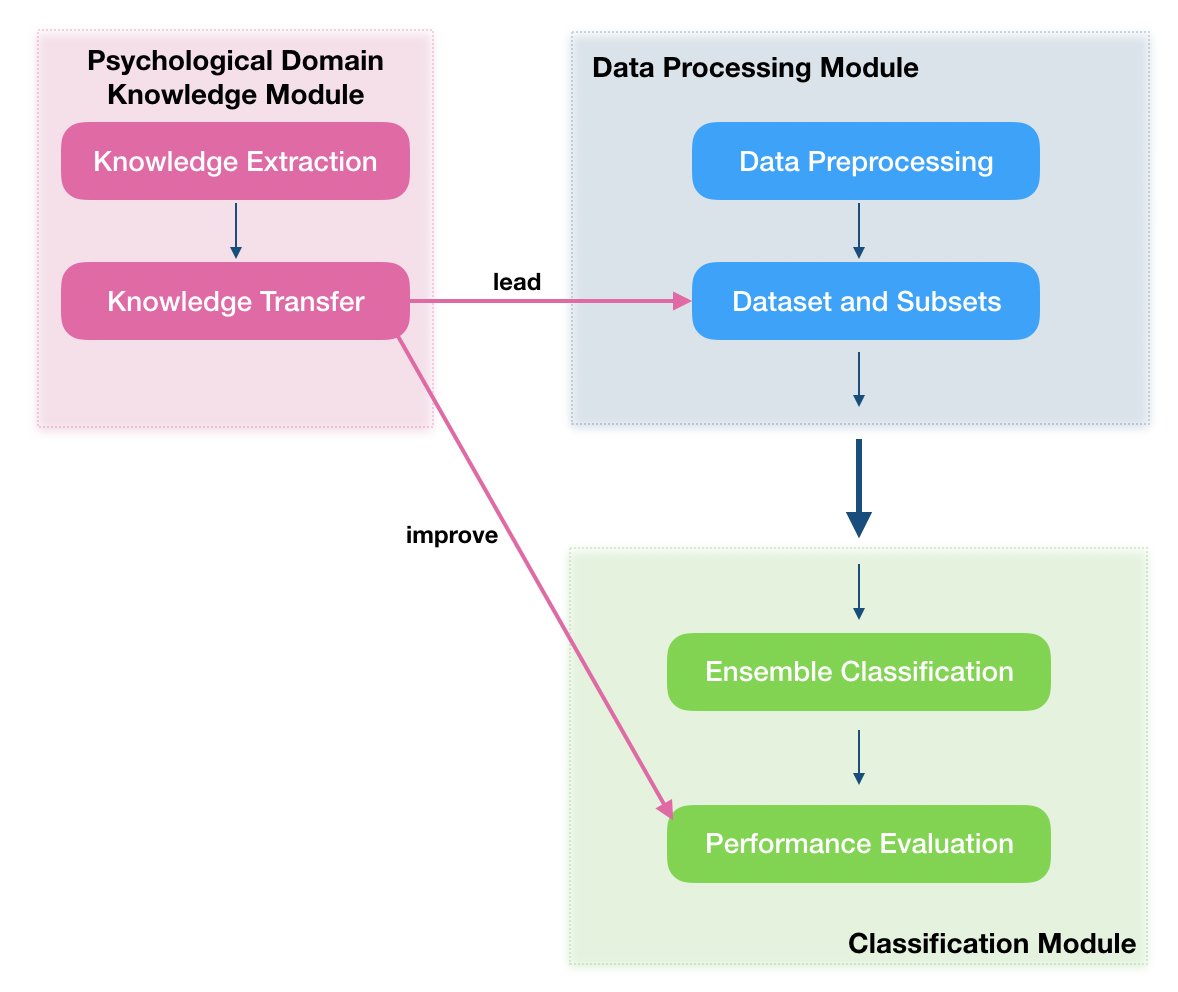
\includegraphics[width=1\textwidth]{concepts.png}
\caption{Conceptual Framework} \label{fig1}
\end{figure}
%
Psychological knowledge module learns the knowledge how to group health informatics in psychological domain. It is a guideline to direct the actions how to transform the dataset in data processing module. It also assists designing ensemble classification technique in classification modelling module. Data processing module contains all proceedings of data preprocessing, feature extraction and dataset establishment. The module converts the data from rare health statistics dataset into several normalised dataset being ready for classification. The last modelling module implements the classification of dataset. It builds an effective ensemble classifier and performs the comparative prediction of depressive risk for participants. 
\\
\medskip

\subsection{Psychological Knowledge}
Kroenke et, al. \cite{Kroenke} discovered that there was a strong association between increasing depression severity screen scores and worsening functionality on all 6 categories: mental, social, role, pain, physical and general functions. These 6 categories were directly interpreted 5 items of mental health diagnostic criteria in Mental Health Inventory (MHI-5) and additionally mental disorder symptoms as mental category. The research illustrated graphically the relationship between increasing PHQ-9 scores of depression and worsening functional categories (see Fig.~\ref{fig2}). 
\begin{figure}[h]
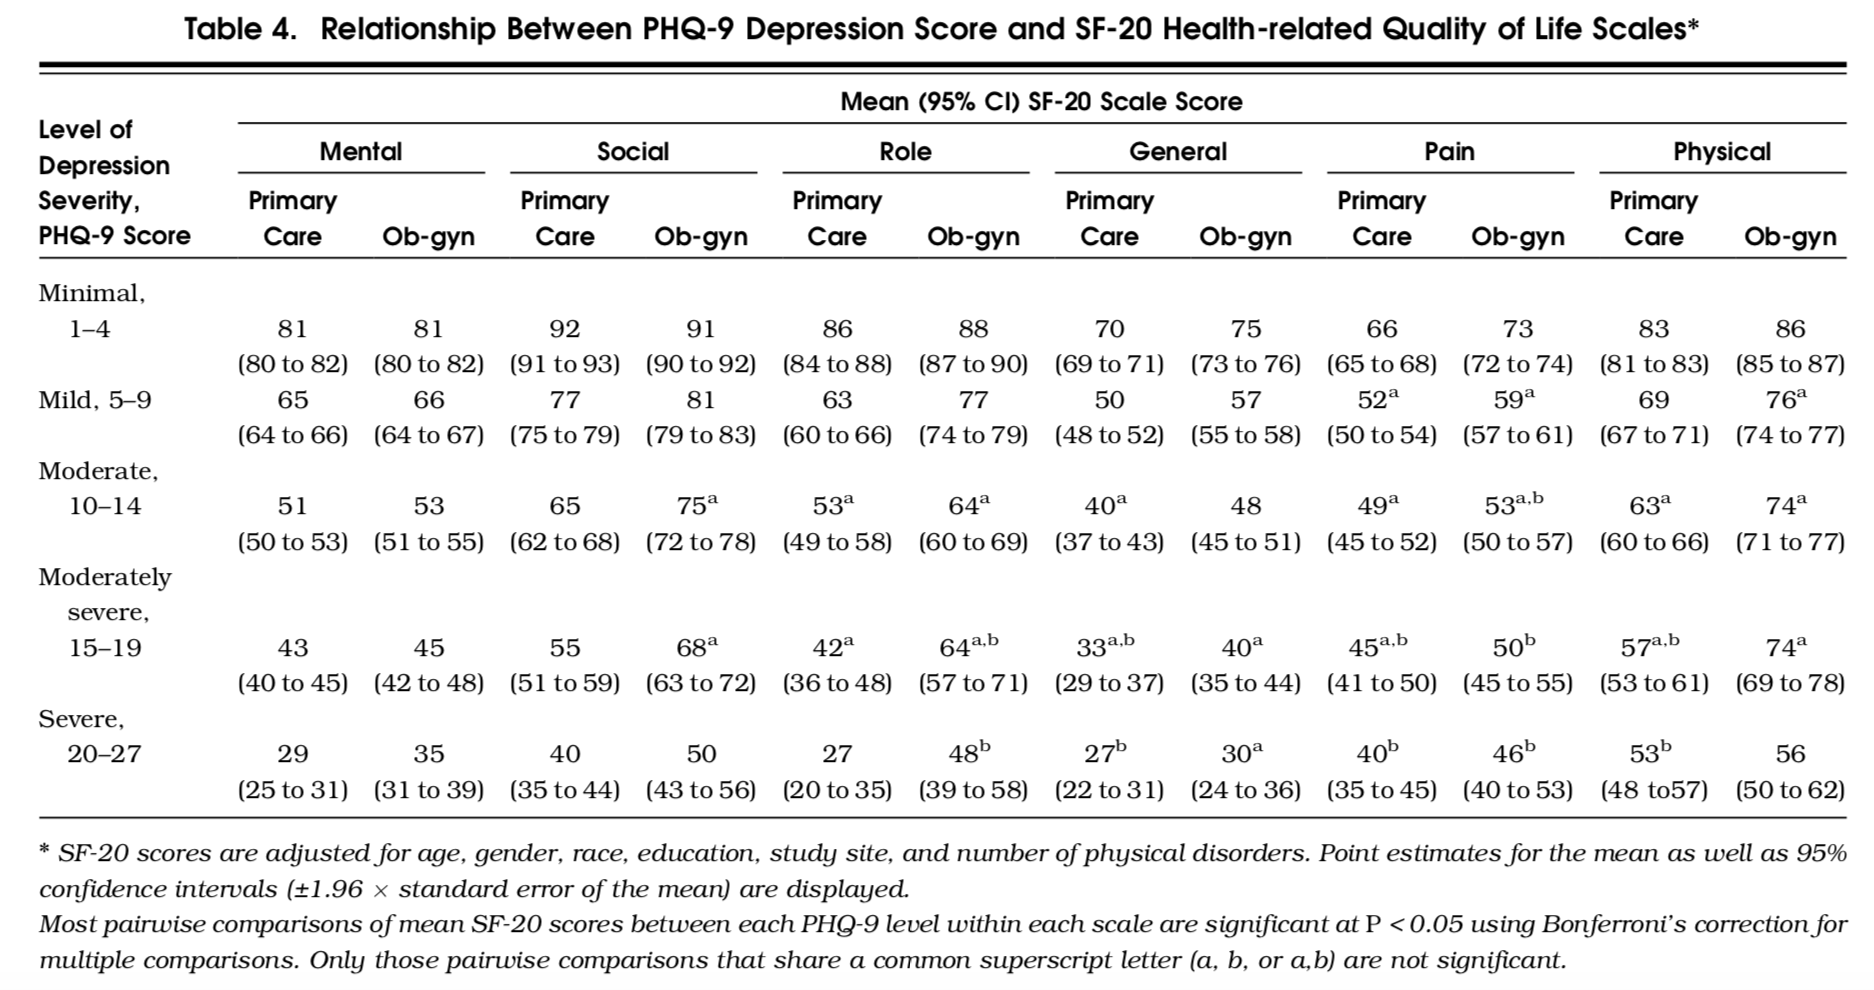
\includegraphics[width=1\textwidth]{phq-9.png}
\caption{The relationship between depression severity and personal health-related functionalities\cite{Kroenke}} \label{fig2}
\end{figure}

Associations of health related functionings with depression have been observed in many previous studies at psychological domain. For instance, Clark et, al. \cite{Clark} explored the opposite association of depression and psychosocial functionings. The research examined the potential psychosocial benefits of wellness coaching in functionings which included the overall quality of life and the 5 domains of physical, social, emotional, cognitive, and spiritual functioning. It found that depression is associated with poor health status and negative health behaviours. It also addressed that participants significantly reduced their level of depression after improving health functional status by wellness coaching. The researchers suggested that additional self-care on physical activity, health sleep, spirituality and social activities could help on long-term depression management. Ostir et, al. \cite{Ostir} discovered that patients identified as not depressed showed greater improvement in functional status than other patient groups in stoke disease.The research varied previous reports on the association between depression and functional status. It suggested that early recognition and management of depression in person with stroke represents an important effort to improve health outcomes and facilitate functional independence. Moreover, Gonzalez-Saenz de Tejada et, al. \cite{Gonzalez-Saenz} explored the association of functional and psychological status of cancer patients. The study addressed that patients with depression showed lower gains in all health related functional domains than patients without depression. It confirmed again that patients with depression tended to show less improvement in all functional variables in health related quality of life (physical, role, emotional, cognitive, and social function, and global quality of life). And it also confirmed that depression were associated with changes in at least one pre-noted functional variable.
\\

By analysis of the relationship between depression and variables of functional status, the scales of health-related functional variables have the similar trend as the severity of depression in statistics. Previous studies in related-work were more focused on detecting depressive symptoms and depression-related contents. Likewise, this relationship innovates a new potential method of predicting users' depression by sampling various diagnostic criteria of functionality. The classification technique and binary ground truth technique will enhance the strength of new type prediction as well. New method apparently has a couple benefits comparing to previous techniques:
\begin{enumerate}[label=\alph*)]
  \item There are more features available for classification due to enlarged inputs in various functional areas;
  \item It is more easier to acquire functional data than sensitive data of depressive symptoms especially on social network; 
  \item It is more easier to cover sufficient specificities of one functional status than to cover all available types of depressive symptoms;
  \item It is more accuracy and more comparable in the classification of six functional status group than in only one collection of depressive symptoms;
  \item It can provide a real opportunity to apply the similar method on automatically detecting depression on social network.
\end{enumerate}

Therefore, we can transfer psychological domain knowledge to information domain. \textit{$\mathbb{D}^s$} can be leveraged and divide into 6 sub-datasets. The dataset of user mental profile need to be redefined:\\
\\
\textbf{Definition 4} Let new redesigned $\mathbb{U}$ = $\langle u_{mental}, u_{social}, u_{role}, u_{pain}, u_{physical}, u_{general} \rangle$, every u  $\in \mathbb{U}$ is an independent function of user, where
\begin{itemize}
  \item $u_{mental}$ presents individual mental disorder symptoms;
  \item $u_{social}$ presents mental diagnostic criteria in the social activities;
  \item $u_{role}$ presents mental diagnostic criteria in the role funcitonlity;
  \item $u_{pain}$ presents mental diagnostic criteria in the pain domain ;
  \item $u_{physical}$ presents mental diagnostic criteria in the physical category;
  \item $u_{general}$ presents mental diagnostic criteria in the general actions.
\end{itemize}
\medskip

\subsection{Data Processing}

In this research, we use the dataset that was directly collected from national health examination survey. It is generally used for health statistics, but unfortunately not for data mining. And we only use the survey question part which was one third of whole dataset. It was organised by variety of health survey questions which divided questions into columns and participants into rows amongst different tables of health domain. Since those tables were not organised in the same format and structure, the pre-processing of them is hence prominent for later classification. 
\\

Data cleaning and transformation is prior in the whole procedure of data preparation because all data should be computer readable and not redundant. And data types in the dataset are justified in order to make each other compatible and comparative. The normalisation is also necessary to uniform the scale condition in various questions. Whilst data preprocessing is implemented, psychological domain knowledge in functional diagnostic criteria is applied in the reconstruction of data structure. According to Definition 4, we can lower the dimension of data set by reducing the number of tables. All tables need to be reconstructed into only six tables referred by six categories of depression diagnostic criteria in functionality (see Fig.~\ref{fig3}).
\begin{figure}[h]
\hspace{2cm}
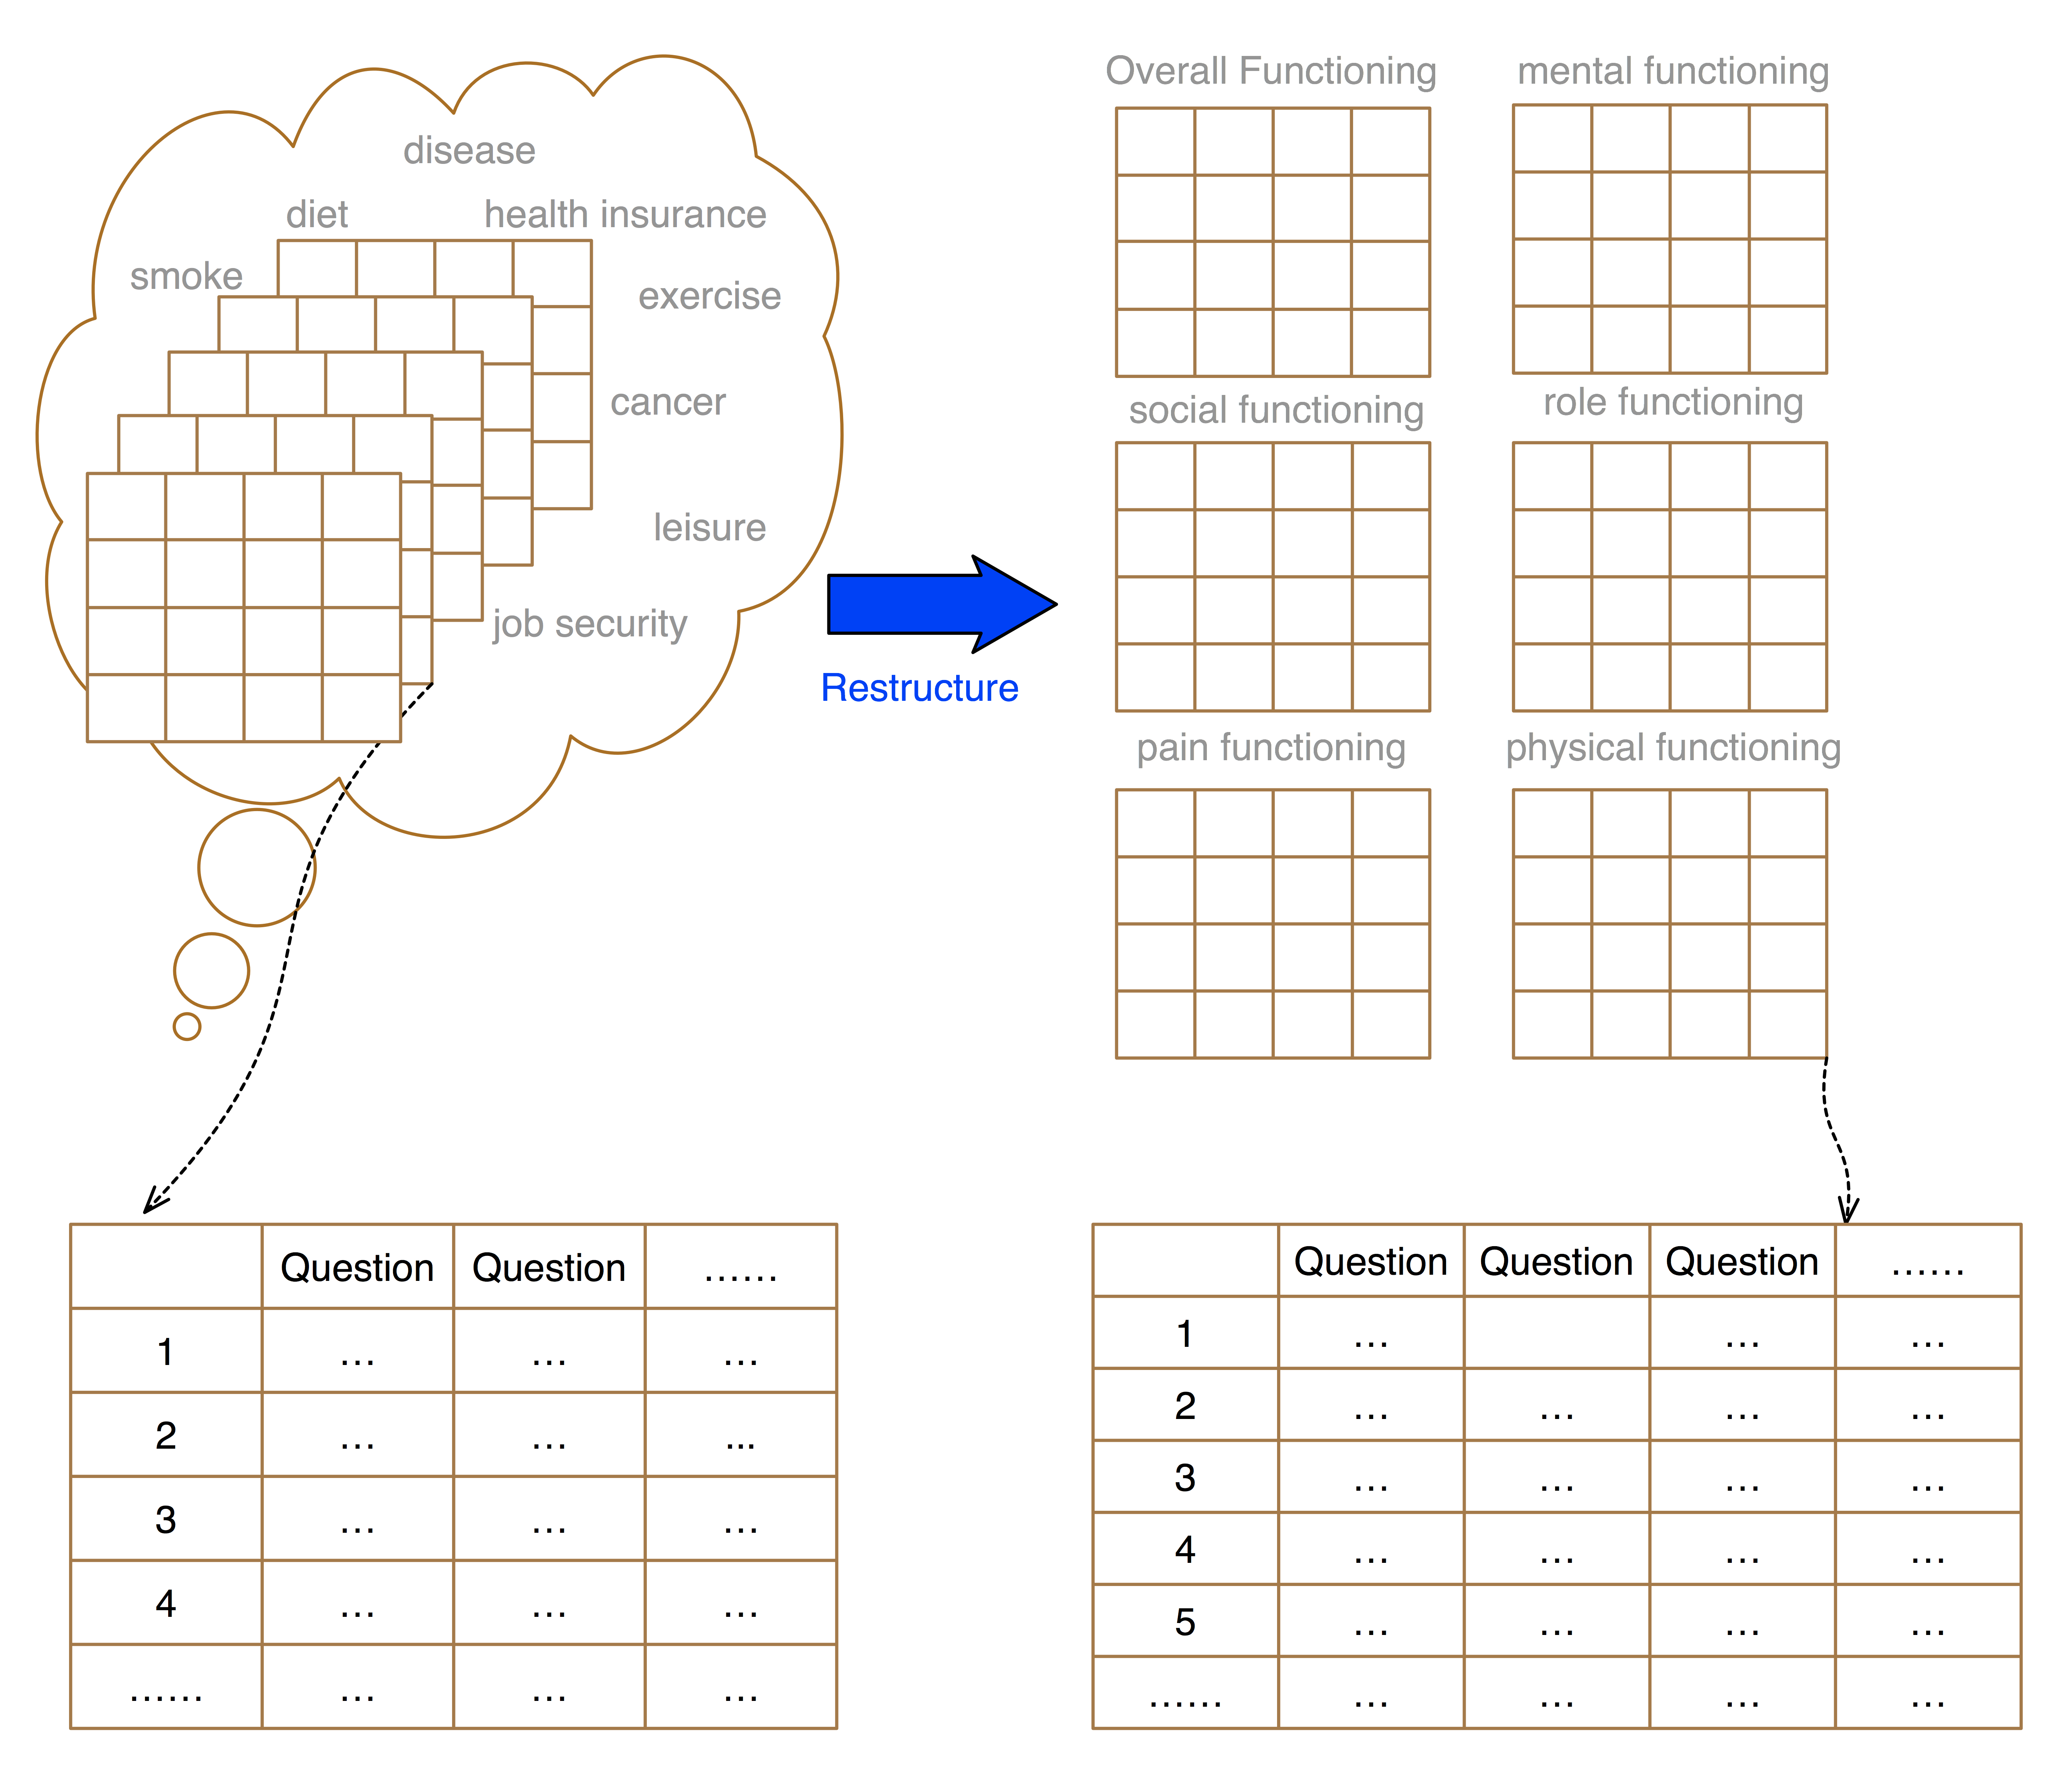
\includegraphics[width=0.6\textwidth]{restructure.png}
\caption{Data Restructure based on Psychological Knowledge Base} \label{fig3}
\end{figure}
They may involve different number of questions but they all have the same participants. Furthermore, those six tables can be rejoin into one big table due to same row index of them. By instant consideration of those tables, each table forms a new dataset where participants are cases and questions are features. We can therefore define the new datasets after data pre-processing as below:\\
\\
\textbf{Definition 5} Let new overall dataset of m cases and n features $\mathbb{D}_{overall}$ = $\displaystyle \big\{ (x_{1}, x_{2}, ... , x_{n}, y ), x_{i} \in R^{m}, y \in {\{0, 1\}}^{m}  \big\}$, and sub-datasets of different 6 functional categories $\mathbb{D}_{mental}$, $\mathbb{D}_{social}$, $\mathbb{D}_{role}$, $\mathbb{D}_{pain}$, $\mathbb{D}_{physical}$ and $\mathbb{D}_{general}$, where
\begin{itemize}
  \item $|\mathbb{D}_{overall}|$ = $|\mathbb{D}_{mental}|$ = $|\mathbb{D}_{social}|$ = $|\mathbb{D}_{role}|$ = $|\mathbb{D}_{pain}|$ = $|\mathbb{D}_{physical}|$ = $|\mathbb{D}_{general}|$ = $m$;
  \item Feature($\mathbb{D}_{mental}$) + Feature($\mathbb{D}_{social}$) + Feature($\mathbb{D}_{role}$) + Feature($\mathbb{D}_{pain}$) + Feature($\mathbb{D}_{physical}$) + Feature($\mathbb{D}_{general}$) = Feature($\mathbb{D}_{overall}$) = n . \\
\end{itemize}

\medskip

\subsection{Modelling}
In this study, we use an ensemble classification approach to build the model for detecting depression. It implements the independent ensemble methodology which applies several classification techniques in parallel. They are Support Vector Machine (SVM) technique, Artificial Neutral Network(ANN) algorithm, K-Nearest Neighbour (KNN) method and Decision Tree (DT) method. Each composite classifier among them is trained on the same portion of the training set in one run. The performance of them are evaluated by k-fold cross validation algorithm. And amalgamating all outputs of composite classifiers into a single prediction, we consequently generates the ensemble classifier. The main idea of this ensemble classification approach is to collect various outputs of multiple independent classifiers and combines them to improve the predictive performance. 
\\

In general, the ensemble method provides higher accuracies and better predictive performance than a single algorithm \cite{Rokach}. There are several reasons why ensemble methods having a better performance \cite{Sagi}: 
\renewcommand\labelitemii{$\square$}
\begin{enumerate}[label=(\roman*)]
  \item Overfitting avoidance: ensemble methods improve the overall predictive performance by averaging different hypothesis to reduce the risk of choosing an incorrect hypothesis.  
  \item \vspace{3mm} Computational advantage: ensemble methods decrease the risk of obtaining a local minimum by combining several learners, ensemble methods.
  \item \vspace{3mm}Strong representation: ensemble methods achieve a better fit to the data space due to combining different models and extending the search space. 
\end{enumerate}

Moreover, ensemble methods are considered the potential solution for several machine learning challenges like class imbalance, concept drift and curse of dimensionality \cite{Sagi}. For example, Lu, Cheung and Tang \cite{Lu} proposed a new ensemble algorithm to utilise both undersampling and oversampling base sampling methods in data training; the proposed method specifically selected various sampling rate for each data set; they also illustrated that the proposed ensemble method significantly outperformed other traditional algorithms for class imbalanced problem. And about concept drift problem, Limsetto and Waiyamai \cite{Limsetto} considered that it can be solved in multiple ways such as robust classifier, data sampling, semi-supervised learning and cost-based learning. They proposed an ensemble method from many well-known models instead of one that resulting in less bias than previous baseline models; and the experimental results demonstrated that the ensemble model yielded better performance when class distribution of data set was not set uniformly. Furthermore, Serpen and Pathical \cite{Serpen} researched how the ensemble method solved curse of dimensionality problem in machine learning; they divided high-dimensional feature space into subspaces and assigned each subspace alongst a base learner within an ensemble machine learning context; their simulation of over 20,000 features indicated that the ensemble classifier had better performance in prediction accuracy and cpu time than other benchmark machine learners. Therefore, ensemble methods are obtained widely to avoid above problems and further improve the overall performance in classification.
\\

The ensemble method also imitates human nature by seeking various solutions before making a final decision \cite{Sagi} and therefore, it becomes a nature option for modelling. The ensemble method hence is considered as a optimised technology comparing to other baseline models in the classification of our pre-processed data.
\\

\subsubsection{Ensemble Model}
After a better understand of the strengths and limitations of each model, the ensemble of integrating four algorithms together is possible to maximum the predictive performance. "The objective is to utilise the strengths of one method to complement the weaknesses of another" \cite{Kotsiantis}. While more specifically each independent sub-model is trained, more targeted concepts are covered by the ensemble classifier and more accuracy it becomes. 
\\

In order to combine all baseline classifiers' outputs, our modelling procedure adopts weighting ensemble method. Weighting ensemble method is very genetic when all base classifiers have uniform comparable outputs. The weight of each classifier can be set proportional to its accuracy performance on a validation set \cite{Rokach}:\\
\begin{equation}\label{reio}
	w_{i} = \frac{1 - E_{i} }{\sum_{k = 1}^{n} (1 - E_{k}) } 
\end{equation}
where $E_{i} $ is a normalisation factor which is based on the predictive performance of classifier $i$ on the validation set. 

In view of the fact that the ensemble classifier combines weighted outputs of all base classifiers, we can define the ensemble classifier as below: \\
\\
\textbf{Definition 6} Let the ensemble model \\
\begin{equation}\label{reio}
	\mathbb{M}_{e} = \sum_{k = 1}^{n} w_{i} M_{i} 
\end{equation}
where
\begin{itemize}
  \item $M_{i}$ presents a single base model;
  \item $w_{i}$ presents the weighting metric of predictive performance at specific base model $M_{i}$;
  \item $k$ is the order of base models;
  \item $n$ is the total number of base models, and in our case $n = 4$;
  \item $i$ is the order number of specific base model.\\
\end{itemize}

In this ensemble method, the driving principle is to build a couple of estimators independently and then to average their predictions. The combined estimator is usually better than any of the single base estimator because instances' variance is moderated.

\subsubsection{Adapted Classification Methods}
Our ensemble classification method involves several baseline supervised classification models. Supervised classification is one of most frequently applications in predictive data mining. We have concentrated on selecting intricate supervised learning algorithms within diverse advantages. The goal of each classification method is to build a concise model to achieve the best possible prediction accuracy. However, each classification method has diverse computing algorithm. There are several most important supervised machine learning techniques \cite{Kotsiantis}:\\
\begin{enumerate}[label=\alph*)]
	\item Logic based algorithm: The algorithms use logic or rules to make a decision of selecting proper features during the learning. Decision tree method adopts this algorithm.
	\item Perceptron-based techniques: The algorithms are based on the notion of perceptron to construct a pattern like layers of neutrons to learn different paths in the classification. Neutral network is its well-known representer.
	\item Statistical learning algorithms: The algorithm uses statistical approaches to provide a probability that an instance belongs in each class. Under this category of classification algorithms, one can find Naive Bayesian network and k-Nearest Neighbour technique.
	\item Support vector machines: Support Vector Machine is the newest supervised machine learning technique \cite{Kotsiantis}. In classic, it uses a hyperplane to separate two data classes and the margin created by the separating hyperplane indicates how the success of classification is. \\
\end{enumerate}

We propose to involve one method of each type in order to present sufficient algorithms in the limited number of sub-models. We thereby select four techniques for baseline models: Decision Tree method, Artificial Neutral Network technique, k-Nearest Neighbour method and Support Vector Machine algorithm.
\\

\textbf{Decision Tree (DT):\\}
Decision trees are logic trees that classify instances by evaluating them based on attributes. Each internal node in a decision tree represents evaluating an attribute in an instance, each branch represents the outcome of evaluation and each leaf node represents a class label. Instances are classified starting at the root node and stop at one leaf node after computing all attributes on the path. Decision tree algorithm is the easiest algorithm and capable of classifying huge datasets \cite{Somvanshi}.
It is simple to understand and interpret. Kotsiantis et, al. \cite{Kotsiantis}addressed that one of the most useful characteristics of decision trees is their comprehensibility, which makes users can easily understand why a decision tree classifies an instance as a specific class label. And decision tree method can make a decision even with little hard data. Somvanshi et, al. \cite{Somvanshi} believed that decision tree algorithm can process the data which contains the missing values and errors. Their research showed that decision tree is able to work very good in the presence of redundant attributes. Likewise, a disadvantage of decision tree method is well-known. The algorithm is unstable that a small change in the data may change the overall look of decision tree. However, decision tree algorithm is still one of the most useful and powerful algorithm in supervised learning. 
\\\\\\

\textbf{Artificial Neutral Network (ANN)\\}
Artificial neutral network is a biologically inspired algorithm to simulate the manner of nerve cells in the brain. According to the book of Kumar \cite{Kumar}, ANN is made up of elements named as artificial neurons; the neurons are organised in network to simulate the anatomy of brain by a standard processing whose output is calculated by multiplying its input by a weight vector; they are aggregated into layers and layers are aggregated into the network to form highly interconnected processing structures; whilst the input layer doesn't process information, it simply sends the inputs, modified by a weight, to each of the neurons in the next layer; and the next layer does the processing which can be a hidden layer or the output layer in a single layer design. ANNs are usually more able to easily provide incremental learning than decision trees as having a good multiple layers architecture. Fei and Li \cite{Fei} discovered that ANN are widely used in medical data mining methodology, and the combination of ANNs and some other algorithms will be able to achieve a better results in medical diagnosis and prediction. Likewise, ANN contains some weaknesses, including "poor general application of the architecture, inaccurate analysis for various indicators of the network and uncontrollable time of machine learning" \cite{Fei}. Kotsiantis et, al. \cite{Kotsiantis}concluded that the most striking disadvantage of ANN is lack of ability to answer how the output in a specific way being effectively communicated. Generally, it is a problem to properly determining the size of the hidden layer. The underestimated neutrons in hidden layer can lead to poor approximation, while "excessive nodes can result in overfitting and eventually make the search for the global optimum more difficult" \cite{Kotsiantis}. In spite of its several disadvantages,  ANN is still a good competitor for other learning algorithms, which has been used on a variety of intricate problems including computer vision, speech recognition, recommendation filtering even medical diagnosis \cite{Somvanshi}\cite{Kumar}.
\\

\textbf{K-Nearest Neighbour (KNN)\\}
Conversely to intricate neutral networks, the K-Nearest Neighbor algorithm is a typical lazy learning algorithms. KNN is based on the principle that classifying instances is to find other similar instances that have proximate properties. "If the instances are tagged with a classification label, then the value of the label of an unclassified instance can be determined by observing the class of its nearest neighbours" \cite{Kotsiantis}.  In KNN assigning weight by the contributions of the neighbours, the nearer neighbours thereby contribute more to the average than other distant ones. This algorithm can be used for both classification and regression. And it is among the simplest machine learning algorithms, even no explicit training step is required. KNN has somewhat weaknesses in computational time and classification accuracy. Though KNN is very sensitive to the choice of the similarity function that is used to compare the contribution of neighbours \cite{Kotsiantis}, it is still a popular classification technique.
\\

\textbf{Support Vector Machine (SVM)\\}
Support Vector Machine algorithm is the newest classification technique among the proposed methods. In classification, SVM constructs a hyperplane or set of hyperplanes in the dimensional space; the hyperplane separates the training data into diverse two classes; and a good classification is achieved by the hyperplane's capability to make a larger margin between two classes of training data. As the application environment is dimensional space, input data of SVM are paired into vectors and vectors are defined in terms of a kernel function. Selection of proper hyperplane and proper parameters for kernel function gives more accurate results as compared to neural networks \cite{Somvanshi}. As the model complexity of an SVM is unaffected by the number of features encountered in the training data, SVM is well suited to deal with learning dataset with large number of features and training instances. Also, choice of an appropriate kernel leads to different SVM applications in linear, nonlinear and multiclass classification. The potential drawbacks of SVM are addressed including \cite{Kotsiantis}: a) requiring full label of input data; b) being difficult to interpret parameters of the solved model; c) being unsuitable for non-binary multiple classification problems.
\\

Meanwhile, Choudhary and Gianey \cite{Choudhary} stated that every learning algorithm differs according to area of application and no algorithm is more powerful than the other in all scenarios. They concluded that the choice of a suitable algorithm depends on the type of problem and the given data, and the accuracy can be improved by using two or more algorithms together. We therefore comprise above four algorithms into ensemble model for this study.

\subsubsection{Algorithm}
Given a well-preprocessed dataset of m examples and n features $\mathbb{D}$ = $\displaystyle \big\{ (x_{1}, x_{2}, ... , x_{n}, y ), x_{i} \in R^{m}, y \in {\{0, 1\}}^{m}  \big\}$, we can generate a suitable ensemble model $\mathbb{M}_{e} $ to present a mapping of $\big\{ x_{1}, x_{2}, ... , x_{n} \big\}$ to $\big\{ y \big\}$ by applying $h$ various types of baseline model $M_{i}$:\\
\IncMargin{2em}
\begin{algorithm}[H]
\SetKwInOut{Input}{input}\SetKwInOut{Output}{output}
\Input{Dataset $\mathbb{D}$ = $\displaystyle \big\{ (x_{1}, x_{2}, ... , x_{n}, y ), x_{i} \in R^{m}, y \in {\{0, 1\}}^{m}  \big\}$}
\Output{Ensemble Model $\mathbb{M}_{e} $}
\BlankLine
Set the training set as $\mathbb{R} = \big\{ (x_{1}, x_{2}, ... , x_{n} ), x_{i} \in R^{m} \big\}$, and the testing set as $\mathbb{S} = \big\{  y, y \in {\{0, 1\}}^{m}  \big\}$\;
\For{$i\leftarrow 1$ \KwTo $h$}{
	\emph{/* validate baseline model */ }\\
	Do training $M_{i}$ on the training set $\mathbb{R}$ \;
	Get the performance $E_{i}$ while validating training result on $\mathbb{S}$ \;
}
Calculate $w_{i} = \frac{1 - E_{i} }{\sum_{k = 1}^{h} (1 - E_{k}) }$; /* calculate performance weightings */\\
Obtain the ensemble model $\mathbb{M}_{e} = \sum_{g = 1}^{h} w_{i} M_{i} $\;
\caption{Ensemble Modelling}\label{ensemble}
\end{algorithm}\DecMargin{2em}


\bigskip
\goodbreak
% =================================================================Experiment
\section{Experiment}
We employ an ensemble supervised learning experiment to classify depressive users from a rare health survey dataset $\mathbb{H}$. We follow psychological knowledge to reduce the dimension of dataset by split dataset into sub-sets. It will not only benefit the processing of classification but also provide a great opportunity to compare the performance of overall dataset and subsets for support of further solution on the real condition with less features.

\subsection{Experiment Design}
In experiment, we first obtain dataset $\mathbb{D}_{overall}$ by data preprocessing on survey data $\mathbb{H}$; next, we aggregate all features of $\mathbb{D}_{overall}$ into 6 health-related functional classes and follow the same procedure to divide $\mathbb{D}_{overall}$ into 6 sub-sets $\mathbb{D}_{physical}$, $\mathbb{D}_{role}$, $\mathbb{D}_{mental}$, $\mathbb{D}_{social}$, $\mathbb{D}_{pain}$ and $\mathbb{D}_{general}$; and we train dataset $\mathbb{D}_{overall}$ by four baseline models (DT, ANN, KNN, SVM) to obtain the relevant performances; then we build the ensemble model $\mathbb{M}_{e}$ by calculating the performance weight $w_{i}$ of each baseline model $M_{i} $; furthermore, we train all 6 sub-datasets by the ensemble classifier $\mathbb{M}_{e}$; and the final step is to use k-fold cross validation algorithm to value the complete predictive performance. The overall look of all experiment proceedings is illustrated in Fig.~\ref{fig4}. 
\begin{figure}[h]
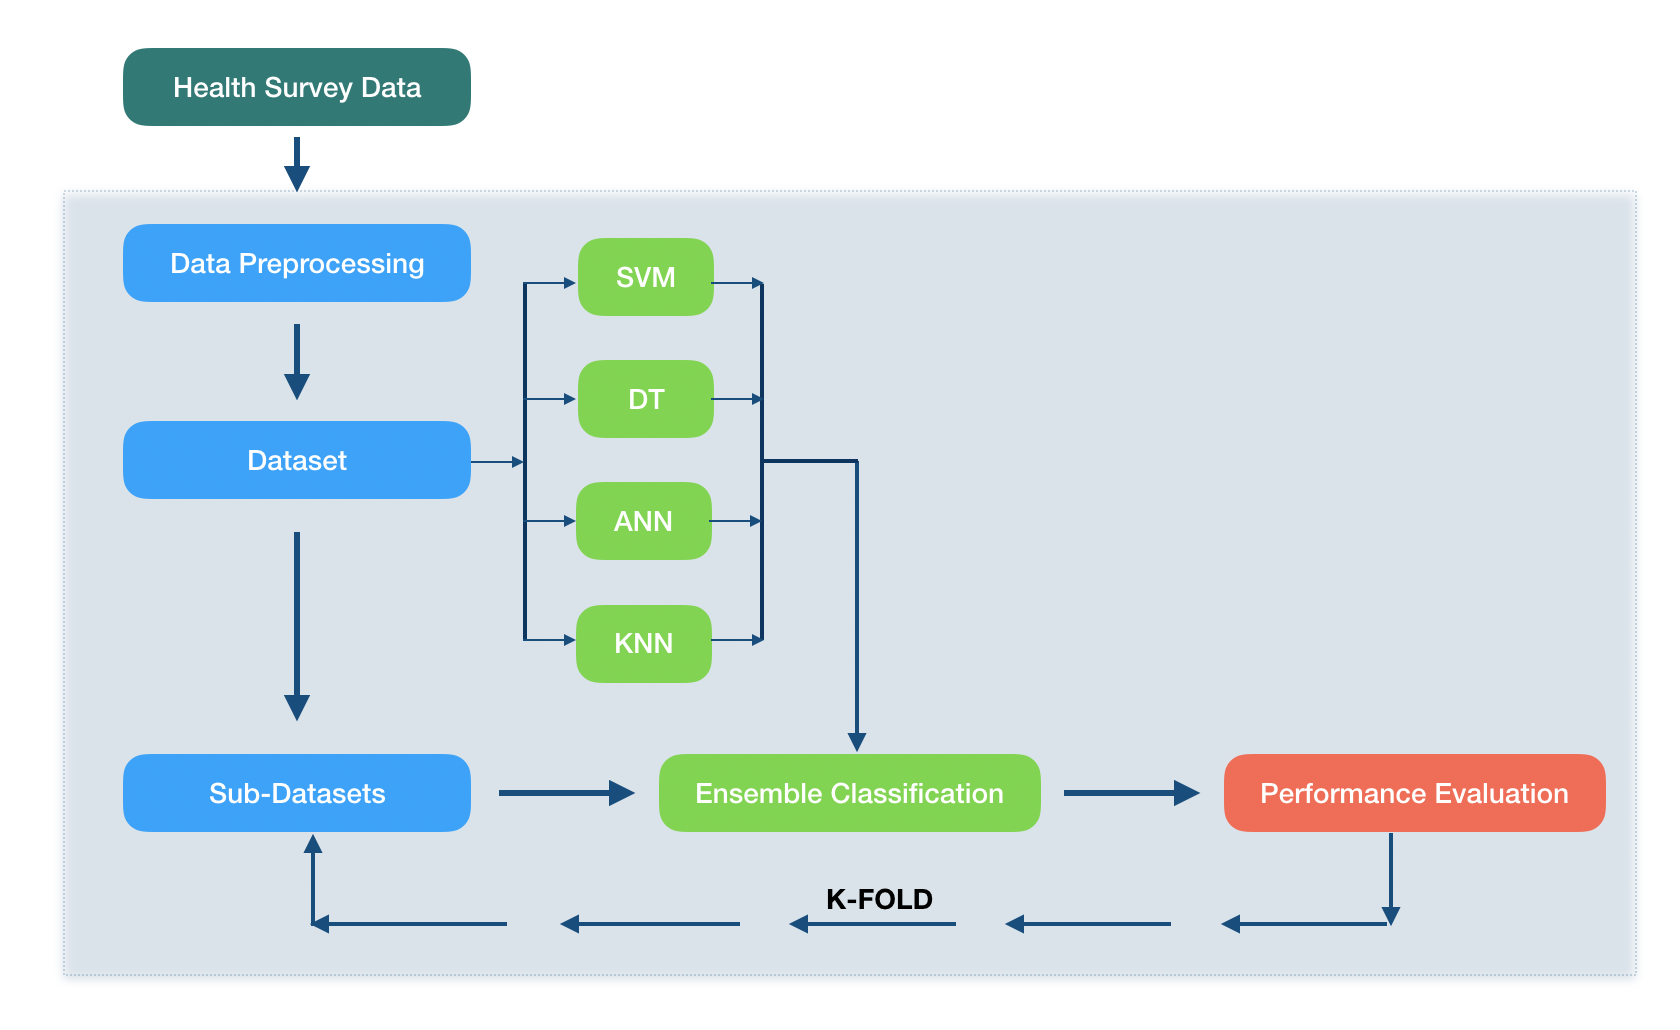
\includegraphics[width=1\textwidth]{experiment.png}
\caption{The overall look of experiment proceedings} \label{fig4}
\end{figure}
\\
\\


From the proceeding details of classification, we can define the algorithm of whole experiment as below: \\\\\\
\IncMargin{2em}
\begin{algorithm}[H]
\SetKwInOut{Input}{input}\SetKwInOut{Output}{output}
\Input{a rare health survey dataset $\mathbb{H}$}
\Output{Ensemble Classifier $\mathbb{F}_{e}$ and the complete prediction}
\BlankLine
Obtain dataset $\mathbb{D}_{o}$ by data pre-processing on survey data $\mathbb{H}$\;
Aggregate features manually referred on 6 psychological functionalities \;
$\mathbb{D}_{o}$ = $\mathbb{D}_{ph}$ $\cup$ $\mathbb{D}_{r}$ $\cup$ $\mathbb{D}_{m}$ $\cup$  $\mathbb{D}_{s}$ $\cup$ $\mathbb{D}_{pa}$ $\cup$ $\mathbb{D}_{g}$, for each pair of ($\mathbb{D}_{i}$, $\mathbb{D}_{j}$), where both $\mathbb{D}_{i}$ and  $\mathbb{D}_{j}$ $\in$ \{$\mathbb{D}_{ph}$, $\mathbb{D}_{r}$, $\mathbb{D}_{m}$, $\mathbb{D}_{s}$, $\mathbb{D}_{pa}$, $\mathbb{D}_{g}$\}, $\mathbb{D}_{i}$ $\cap$ $\mathbb{D}_{j}$ = $\phi$\;
Supervised learning on $\mathbb{D}_{overall}$ for ensemble model $\mathbb{M}_{e} = \sum_{g = 1}^{h} w_{i} M_{i} $\;
\ForEach{sub-dataset $\mathbb{D}_{i}$ in \{$\mathbb{D}_{o}, \mathbb{D}_{ph}$, $\mathbb{D}_{r}$, $\mathbb{D}_{m}$, $\mathbb{D}_{s}$, $\mathbb{D}_{pa}$, $\mathbb{D}_{g}$\}}{
	\emph{/* ensemble classification*/}\\
	Do ensemble classification on  $\mathbb{D}_{i}$ \;
	Validate its predictive performance\;
}
\caption{Experiment Design}\label{experiment}
\end{algorithm}\DecMargin{2em}

\bigskip
\bigskip
The ensemble classification can be expressed in algorithm as well: Given a well-preprocessed dataset of m examples and n features $\mathbb{D}$ = $\displaystyle \big\{ (x_{1}, x_{2}, ... , x_{n}, y ), x_{i} \in R^{m}, y \in {\{0, 1\}}^{m}  \big\}$, we can obtain the ensemble classifier $\mathbb{F}_{e}$ = $w_{svm} \cdot f_{svm}$ + $w_{nb} \cdot f_{nb}$ + $w_{knn} \cdot f_{knn}$ + $w_{dt} \cdot f_{dt}$ by applying supervised learning on dataset $\mathbb{D}$:\\
\IncMargin{2em}
\begin{algorithm}[H]
\SetKwFunction{Median}{Median}
\SetKwInOut{Input}{input}\SetKwInOut{Output}{output}
\Input{Dataset $\mathbb{D}$ = $\displaystyle \big\{ (x_{1}, x_{2}, ... , x_{n}, y ), x_{i} \in R^{m}, y \in {\{0, 1\}}^{m}  \big\}$}
\Output{the optimised ensemble classifier $\mathbb{F}_{e} $ and its predictive performance $p_{e}$ }
\BlankLine
Divide dataset $\mathbb{D}$ into k portions, each portion has $\frac{m}{k}$ examples\;
\For{$k\leftarrow 1$ \KwTo 5}{ 
	Select all portions except $k^{th}$ portion to form new dataset $\mathbb{D}^{'}$ \;
	Use $\mathbb{D}^{'}$ to generate the training set $\mathbb{R} = \big\{ (x_{1}, x_{2}, ... , x_{n} ) \big\}$ and the testing set $\mathbb{S} = \big\{  y \big\}$, where $|\mathbb{D}^{'}| = |\mathbb{R}| = |\mathbb{S}| = \frac{4}{5}|\mathbb{D}| = \frac{4m}{5}$\;
	\emph{/* baseline model */}\\
	\ForEach{ one classification method of SVM, ANN, KNN, DT}{ 
		Training on the training set $\mathbb{R}$ and obtain classifier $f$\;
		 Obtain predictive value $y^{p} = f(\sum_{i=1}^{n} (x_{i}))$ \;
	}
	\emph{/* ensemble */}\\
	Calculate the ensemble classifier $\mathbb{F}_{k}$ = $w_{svm} \cdot f_{svm}$ + $w_{nb} \cdot f_{nb}$ + $w_{knn} \cdot f_{knn}$ + $w_{dt} \cdot f_{dt}$ \;
	Calculate a float predictive value $y_{e}$ = $w_{svm} \cdot y_{svm}^{p}$ + $w_{nb} \cdot y_{nb}^{p}$ + $w_{knn} \cdot y_{knn}^{p}$ +$w_{dt} \cdot y_{dt}^{p}$ \;
	\emph{/* sensitivity */}\\
	\eIf{$y_{e} > 0.5$}{
		$y_{e} = 1$ \emph{/* non-depression */}
	}{
		$y_{e} = 0$ \emph{/* depression */}
	}
	Test $y_{e}$ on testing set $\mathbb{S}$ and report predictive performance $p_{k}$ \;
}
\emph{/* 5-fold cross validation */}\\
Validate the predictive performance by calculating $\displaystyle p_{e} = \frac{\sum_{k=1}^{5} p_{k}}{5}$ \;
Generate the optimised ensemble classifier \hspace{6cm} $\mathbb{F}_{e}$ = Median($\mathbb{F}_{1}, \mathbb{F}_{2}, \mathbb{F}_{3}, \mathbb{F}_{4}, \mathbb{F}_{5}$)
\caption{Ensemble Classification Procedure}\label{classification}
\end{algorithm}\DecMargin{2em}
\medskip

\subsection{Dataset}
\subsubsection{NHANES Survey Data}
\paragraph{}
In this study, we use dataset of National Health and Nutrition Examination Survey (NHANES). NHANES is a population-based survey designed to collect health-related information of the U.S. household population. It is a very rich resource for health professionals and researchers to expand our knowledges of various modern health problems. It is conducted by the National Center for Health Statistics (NCHS), which is part of the Centers for Disease Control and Prevention (CDC). All information in NHANES are gathered and protected with the requirement of Federal Law of U.S. and for health research purposes only. Collections of NHANES in last decade are all free for researchers and published on the website of NCHS.
\\

We employ the questionnaire data in NHANES 2013 - 2014 collection as input data $\mathbb{H}$ of experiment. We also limit the age of participants to 18+ because data of teenage and children are only partially published. As our objective is to classify general person into healthy and depressive groups, the features only involved with single gender are excluded.  
\\
\smallskip

\subsubsection{Build Ground Truth}
NHANES integrates health tools for measuring health status like Patient Health Questionnaire ( PHQ-9 ) depression screen tool. PHQ-9 tool is a 9-item screening instrument to measure depressive severity from no depression to major depressive disorder. In NHANES, PHQ-9 measure is the only integrated measurement for depression because it is a simple, reliable and valid measure of depression severity \cite{Kroenke}. And it has been a useful clinical and research tool in years. There are plenty of health researches assigning with NHANES data and integrated PHQ-9 tool to study depression related health issues. For instance, Tedders et, al. \cite{Tedders} in 2011 researched the relationship between depression and low cholesterol among household population using NHANES data; Merikangas et, al. \cite{Merikangas} in 2012 proposed a association between major depressive disorder and obesity by assessing 2001-2004 NHANES collections; Ubani and Zhang \cite{Ubani} in 2015 published a research of NHANES data to study the role of adiposity in the relationship between serum leptin and severe major depressive episode; and Andrea et, al. \cite{Andrea} in 2016 explored depressed adults information in social support and health service use of NHANES data; Nguyen et, al. \cite{Nguyen} in 2017 research the association between blood folate concentrations and depression in reproductive aged U.S. women in NHANES 2011 - 2012 collection.
\\

Based on the integrated PHQ-9 screen measurement, we can establish ground-truth label information (on whether or not participant has depression) for whole dataset. In scales of PHQ-9 measurement, there are five level of depression severity from minimal level to severe level. In the research of Kroenke et, al. \cite{Kroenke}, they found that patients who were identified at least on the moderate level (score $\geq$ 10) of depression in PHQ-9 measurement had a sensitivity of 88\% and a specificity of 88\% for major depression. We thereby choose the separation at PHQ-9 score 10. Participant who has a PHQ-9 score less than 10 is considered as a healthy person of depression or vice versa. We label these depression-less people as the logical truth or "1"; reversely those depressive people as the logical false or  "0".
\\
\smallskip

\subsubsection{Principles Of Data Preprocessing}
In spite of the fact that NHANES questionnaire collection was very organised and carefully preserved, it still existed some errors and missing values. And naturally part of participants did not complete all questions in the questionnaire. Furthermore,  the questionnaire involves "Refuse" option and "Don't Know" option for nearly every question, because the design of it toke a very cautious consideration of personal privacy and individual interests. It is hence essential to fill, correct and normalise those meaningless inputs. In order to uniform all actions taken in data cleaning, we design a couple of presumption and principles to manage the proceeding:
\begin{enumerate}[label=\alph*)]
	\item	  we assume that missing inputs belong to the persons who have on depressive risk;
	\item   the choice of "Refuse" option or "Don't Know" option is presumed normal which can be corrected by the statistical mean of inputs;
	\item	  all inputs of survey questions should be converted into binary, range and numbers due to the design of answer options;
	\item	  the final value of each input should be normalised and have a limited byte size.\\
\end{enumerate}
\smallskip

\subsubsection{The Overall Dataset}
After data preprocessing, we has an overall dataset that involves 5398 participants with 516 ( 9.56\% ) depressive persons and 4882 ( 90.44\% ) depression-less people among. The features are directly converted from the original major questions in the health survey, which means a major question of NHANES simply presents one feature in our dataset. After rejecting several irrelevant questions that limited by the age or gender, we get a total of 98 features. Among them, inputs in 49 feature are binary, 36 features are range data and the rest 14 features are float numbers. 
\\
\medskip

\subsection{Baseline Models}
Many machine learning packages and tools are accessible to implement common classification algorithms. Scikit-learn library from Python is one of the most well-designed machine learning package. It provides simple and efficient tools for data mining and data analysis. And it nearly contains all supervised learning methods for both binary and multi-class classification. We thereby choose Scikit-learn Python package to implement four baseline models.

\subsubsection{Kernel and Parameters}
How to select suitable kernel and parameters is common task for classification but it is also complex for specific examples. We only balance the settings of baseline models instead searching a perfect for the parameter because it is uncertain if the settings could maximum the performance in utter instances. And the predictive performance is expected being improved by ensemble classification. Therefore, we employ common values for kernel and parameters in four sub-models:\\

\textbf{Decision Tree}:
		\begin{description} 
		\item \hspace{0.5cm} Scikit-learn uses an optimised version of the CART decision tree algorithm; 
		 the depth of the tree is limited at maximum of 3 in order to prevent overfitting; 
		 "min\_samples\_leaf=1" is often the best choice due to few classes in classification; 
		 the criteria of the quality of split is default as the Gini impurity; 
		 sample weight is preferred by normalising the sum of the sample weights to prevent the tree from being biased toward the dominant class.\\
		\end{description} 

	\textbf{Artificial Neutral Network}:
	\begin{description} 
		\item \hspace{0.5cm} ANN model implements a multi-layer perception algorithm within back-propagation training method; 
		 there are three hidden layers in the proposed network and each of them exists 30 neutrons;
		 activation function for the hidden layer is the rectified linear unit function; 
		 Adam stochastic gradient-based optimiser is preferred due to relatively large amount of training samples; 
		 the learning is initialised from a small step-size 0.001 for a reasonably big learning rate;	
		 maximum number of iterations is set as 10000 to prevent run out of memory while doing convergence; 
		 the seed is randomly generated by random state computer generator to achieve the maximum of variability.\\
	\end{description}
	
	\textbf{K-Nearest Neighbour}: 
	\begin{description} 
		 \item \hspace{0.5cm} We use the basic nearest neighbours classifier with k is an integer 5; 
		 the contribution of neighbours is treated equal so the weights between neighbours is set as "uniform"; 
		 the algorithm used to compute the nearest neighbours is set as \"auto\" because the number of features is varied in overall dataset and sub-datasets;
		 the size of leaf is default as 30 which may affect the speed of construction and query; 
		 the default metric is Euclidean due to standard metric configuration.\\\\
	\end{description}
	
	\textbf{Support Vector Machine}: 
	\begin{description} 
		 \item \hspace{0.5cm} A popular Radial Basis Function (RBF) kernel is used in SVM sets; 
		  the parameter \"C\" that trades off misclassification of training examples against simplicity of the decision surface is set as 1; 
		  the parameter \"gamma\" defines how much influence a single training example has is set as "0.1". 
	\end{description}

Moreover, all four base models are configured for binary classification and their predictive performances are weighted in both labelled classes. 
\medskip
%
%
\subsection{Performance Measure}
The predictive performance of each base classifier in our model is evaluated by F1 score which is generated on confusion matrix of validation. In confusion matrix, we simply let the number of real mental healthy cases in the training set as \textbf{condition positive (P)} and let the number of real depressive cases in the training set as  \textbf{condition negative (N)}. And four derivations are defined to make it clear if the classifier is confusing binary classes (P and N):  \\
\begin{enumerate}[label=(\roman*)]
\item let the number of cases where the classifier correctly predicts P as \textbf{ true positive (TP)}
\item let the number of cases where the classifier correctly predicts N as \textbf{true negative (TN)}
\item let the number of cases where the classifier incorrectly predicts P as \textbf{false positive (FP)}
\item let the number of cases where the classifier incorrectly predicts N as \textbf{false negative (FN)}
\end{enumerate}

And four following terminologies are hence defined as below:
\begin{enumerate}[label=\alph*)]
\item \textbf{ Recall or True Positive Rate (TPR)}: \\ 
		\begin{center} $\displaystyle TPR = \frac{TP}{TP + FN} $ \end{center}
\item \textbf{Specificity or True Negative Rate (TNR)}: \\ 
		\begin{center} $\displaystyle TNR = \frac{TN}{TN + FP} $ \end{center}
\item \textbf{Precision or Positive Predictive Value (PPV)}: \\
		\begin{center} $\displaystyle PPV = \frac{TP}{TP + FP} $ \end{center}
\item \textbf{Accuracy (ACC)}: \\ 
		\begin{center} $\displaystyle ACC = \frac{TP + TN}{TP + TN + FP + FN} $\\ \end{center} 
\end{enumerate}

Based on these terminologies, F1 score is a balanced measure of both the precision (PPV) and the recall (TPR) of the validation: 
\begin{equation}\label{reio}
	F1 = \frac{2 }{\frac{1}{TPR} + \frac{1}{PPV}} = \frac{2TP}{2TP + FP + FN}
\end{equation}
Referred to normalisation factor $E$ in equation (1), F1 score need to be normalised first and then is applied to equation (1) to calculate the weight fo each base classifier. 
\\
\bigskip
\goodbreak

% =================================================================Results and Discussion
\section{Results and Discussions}
\subsection{Experimental Results}
By comparing the performances of four base models (illustrated in table. 1), Decision tree algorithm has the highest accuracy and F1 measure. SVM technique has a similar performance as decision tree algorithm but only a bit lagging in precision. ANN method performs more advantageous in precision score and KNN method operates more fitting in recall measure. Almost F1 scores and recall measures are significant in correlation ( $\geq$ 95\%). However, baseline models perform less satisfied in accuracy and precision. 
\begin{table}[ht]
\begin{tabular}{|C{2cm}|C{2cm}|C{2cm}|C{2cm}|C{2cm}|}
\hline
\rowcolor[HTML]{FFFFC7} 
{\color[HTML]{333333} \textbf{Models}} & {\color[HTML]{333333} \textbf{Accuracy (mean)}} & {\color[HTML]{333333} \textbf{Precision (mean)}} & {\color[HTML]{333333} \textbf{Recall (mean)}} & {\color[HTML]{333333} \textbf{F1 score (mean)}} \\ \hline
\rowcolor[HTML]{ECF4FF} 
\textbf{SVM}  & 0.921  & 0.927 & 0.990  & \textbf{0.958}  \\ \hline
\rowcolor[HTML]{ECF4FF} 
\textbf{ANN} & 0.905 & \textbf{0.941} & 0.955 & 0.948 \\ \hline
\rowcolor[HTML]{ECF4FF} 
\textbf{KNN}  & 0.908   & 0.913  & \textbf{0.993}  & 0.951  \\ \hline
\rowcolor[HTML]{ECF4FF} 
\textbf{DT} & \textbf{0.925}  & 0.938 & 0.981  & \textbf{0.959}  \\ \hline
\end{tabular}
\caption{Performances of sub-models in the overall dataset}
\label{submodels}
\end{table}

\subsubsection{Performance of Ensemble Classifier}
We use F1 measure for the main indicator of model's performance. According to equation (1) and (2), we can calculate the weight for each base model (see at table 2.) and further generate the complete form of ensemble classifier:
\begin{equation}
\mathbb{F}_{k} = 0.228 \cdot f_{svm} + 0.283 \cdot f_{nb} + 0.266 \cdot f_{knn} + 0.223 \cdot f_{dt}
\end{equation}
\begin{table}[ht]
\begin{tabular}{|C{3cm}|C{3cm}|C{3cm}|C{3cm}|}
\hline
\rowcolor[HTML]{FFFFC7} 
{\color[HTML]{333333} \textbf{Models}} & {\color[HTML]{333333} \textbf{F1 score (mean)}} & {\color[HTML]{333333} \textbf{1 - F1}} & {\color[HTML]{333333} \textbf{Weight}} \\ \hline
\rowcolor[HTML]{ECF4FF} 
\textbf{SVM}& 0.958  & 0.042  & 0.228 \\ \hline
\rowcolor[HTML]{ECF4FF} 
\textbf{ANN} & 0.948  & 0.052   & \textbf{0.283}    \\ \hline
\rowcolor[HTML]{ECF4FF} 
\textbf{KNN} & 0.951   & 0.049  & 0.266 \\ \hline
\rowcolor[HTML]{ECF4FF} 
\textbf{DT}  & 0.959  & 0.041  & 0.223  \\ \hline
\end{tabular}
\caption{Calculation of weights for sub-models}
\label{weight}
\end{table}

We use F1 score and accuracy measure as the main predication indicators of the ensemble classification. As features and specificity of the overall dataset and each sub-datasets varied, the divided performances are expected (see table.3). Unsurprisingly, ensemble classifier performs better in the overall dataset and mental sub-set. Performances in other sub-sets is compromised in this experiment but is still comparable to other machine learning methodologies \cite{Fatima}\cite{Hassan}\cite{Peng}\cite{Reece}. As DT performs best (0.925 in Accuracy) in the sub-models and ensemble model has a overall Accuracy of 0.954, the improvement $I$ for detecting depression in ensemble classifier is calculated as below (let percentage of depressed instances as $N_{0}$):\\
\begin{equation}\label{reio}
	 I = \frac{Accuracy_{new} - Accuracy_{old}}{N_{0}} = \frac{0.954 - 0.925}{9.56\%} \cdot 100\% = 30.3\%
\end{equation}
Therefore, the proposed ensemble approach increases the predictive performance by 30.3\% for distinguishing depression from non-depressed participants.

\begin{table}[ht]
\begin{tabular}{|C{3cm}|C{3cm}|C{3cm}|C{3cm}|}
\hline
\rowcolor[HTML]{FFFFC7} 
{\color[HTML]{333333} \textbf{Dataset}} & {\color[HTML]{333333} \textbf{Features}} & {\color[HTML]{333333} \textbf{F1 score}} & {\color[HTML]{333333} \textbf{Accuracy}} \\ \hline
\rowcolor[HTML]{ECF4FF} 
\textbf{$\mathbb{D}_{overall}$}& 98  & \textbf{0.976}  & \textbf{0.954} \\ \hline
\rowcolor[HTML]{ECF4FF} 
\textbf{$\mathbb{D}_{physical}$}& 7  & 0.964  & 0.931 \\ \hline
\rowcolor[HTML]{ECF4FF} 
\textbf{$\mathbb{D}_{role}$} & 9  & 0.963   & 0.929    \\ \hline
\rowcolor[HTML]{ECF4FF} 
\textbf{$\mathbb{D}_{social}$} & 6   & 0.964  & 0.931 \\ \hline
\rowcolor[HTML]{ECF4FF} 
\textbf{$\mathbb{D}_{mental}$ }  & 4  & \textbf{0.975}  & \textbf{0.953}  \\ \hline
\rowcolor[HTML]{ECF4FF} 
\textbf{$\mathbb{D}_{pain} $ }  & 2  & 0.961  & 0.925  \\ \hline
\rowcolor[HTML]{ECF4FF} 
\textbf{$\mathbb{D}_{general}$ }  & 70  & 0.964  & 0.931  \\ \hline
\end{tabular}
\caption{Features and performances of ensemble classifier}
\label{subsets}
\end{table}

\subsubsection{The Depressive Prediction}
F1 score is a weighted harmonic mean of precision and recall such that the best score is 1.0 and the worst is 0.0. F1 measure equally considers both precision and recall in the performance measurement. By the comparison of F1 measures in both different algorithms and datasets (see table. 4), ensemble method has a better F1 score than other baseline algorithms. The overall dataset and mental subset enable to be distinguished from other datasets due to a higher level of F1 measures.
\begin{table}[ht]
\begin{adjustwidth}{-1.5cm}{}
\begin{tabular}{|C{2cm}|C{1.5cm}|C{2cm}|C{1.5cm}|C{1.5cm}|C{1.5cm}|C{1.5cm}|C{2cm}|}
\hline
\rowcolor[HTML]{FFFFC7} 
{\color[HTML]{333333} \textbf{Models}} & {\color[HTML]{333333} \textbf{Overall (mean)}} & {\color[HTML]{333333} \textbf{Physical (mean)}} & {\color[HTML]{333333} \textbf{Role (mean)}} &{\color[HTML]{333333} \textbf{Social (mean)}} & {\color[HTML]{333333} \textbf{Mental (mean)}} & {\color[HTML]{333333} \textbf{Pain (mean)}} & {\color[HTML]{333333} \textbf{General (mean)}} \\ \hline
\rowcolor[HTML]{ECF4FF} 
\textbf{SVM} & 0.9577  & 0.950 & 0.950  & 0.950  & 0.957  & 0.950 & 0.951 \\ \hline
\rowcolor[HTML]{ECF4FF} 
\textbf{ANN} & 0.948  & 0.944  & 0.935  & 0.942 & 0.961 & 0.950 & 0.930 \\ \hline
\rowcolor[HTML]{ECF4FF} 
\textbf{KNN} & 0.951  & 0.947 & 0.945 & 0.944 & 0.958 & 0.938 & 0.949 \\ \hline
\rowcolor[HTML]{ECF4FF} 
\textbf{DT} & 0.959 & 0.950  & 0.949 & 0.950  & 0.960  & 0.950 & 0.950  \\ \hline
\rowcolor[HTML]{9AFF99} 
\textbf{Ensemble}  & \textbf{0.976}  & 0.964  & 0.963  & 0.964 & \textbf{0.975} & 0.961 & 0.964  \\ \hline
\end{tabular}
\caption{Performance in F1 score}
\label{F1}
\end{adjustwidth}
\end{table}
\begin{table}[ht]
\begin{adjustwidth}{-1.5cm}{}
\begin{tabular}{|C{2cm}|C{1.5cm}|C{2cm}|C{1.5cm}|C{1.5cm}|C{1.5cm}|C{1.5cm}|C{2cm}|}
\hline
\rowcolor[HTML]{FFFFC7} 
{\color[HTML]{333333} \textbf{Models}} & {\color[HTML]{333333} \textbf{Overall (mean)}} & {\color[HTML]{333333} \textbf{Physical (mean)}} & {\color[HTML]{333333} \textbf{Role (mean)}} &{\color[HTML]{333333} \textbf{Social (mean)}} & {\color[HTML]{333333} \textbf{Mental (mean)}} & {\color[HTML]{333333} \textbf{Pain (mean)}} & {\color[HTML]{333333} \textbf{General (mean)}} \\ \hline
\rowcolor[HTML]{ECF4FF} 
\textbf{SVM} & 0.921  &0.904 & 0.904 & 0.904 & 0.919 & 0.904  & 0.907  \\ \hline
\rowcolor[HTML]{ECF4FF} 
\textbf{ANN} & 0.905 & 0.895 & 0.879 & 0.892 & 0.928 & 0.904 & 0.873 \\ \hline
\rowcolor[HTML]{ECF4FF} 
\textbf{KNN} & 0.908  & 0.900 & 0.896 & 0.895 & 0.923 & 0.886 & 0.904 \\ \hline
\rowcolor[HTML]{ECF4FF} 
\textbf{DT} & 0.924 & 0.905 & 0.904  & 0.905 & 0.926 & 0.904 & 0.906 \\ \hline
\rowcolor[HTML]{9AFF99} 
\textbf{Ensemble} & \textbf{0.954} & 0.931 & 0.929  & 0.931  & 0.953 & 0.925 & 0.931  \\ \hline
\end{tabular}
\caption{Performances of Accuracy}
\label{Accuracy}
\end{adjustwidth}
\end{table}
\begin{table}[ht]
\begin{adjustwidth}{-1.5cm}{}
\begin{tabular}{|C{2cm}|C{1.5cm}|C{2cm}|C{1.5cm}|C{1.5cm}|C{1.5cm}|C{1.5cm}|C{2cm}|}
\hline
\rowcolor[HTML]{FFFFC7} 
{\color[HTML]{333333} \textbf{Models}} & {\color[HTML]{333333} \textbf{Overall (mean)}} & {\color[HTML]{333333} \textbf{Physical (mean)}} & {\color[HTML]{333333} \textbf{Role (mean)}} &{\color[HTML]{333333} \textbf{Social (mean)}} & {\color[HTML]{333333} \textbf{Mental (mean)}} & {\color[HTML]{333333} \textbf{Pain (mean)}} & {\color[HTML]{333333} \textbf{General (mean)}} \\ \hline
\rowcolor[HTML]{ECF4FF} 
\textbf{SVM} & 0.927 & 0.904 & 0.904  & 0.904  & 0.921  & 0.904  & 0.907  \\ \hline
\rowcolor[HTML]{ECF4FF} 
\textbf{ANN}   & 0.941   & 0.919   & 0.911  & 0.917   & 0.939 & 0.904 & 0.924 \\ \hline
\rowcolor[HTML]{ECF4FF} 
\textbf{KNN} & 0.913 & 0.915 & 0.907  & 0.913 & 0.938 & 0.913  & 0.908  \\ \hline
\rowcolor[HTML]{ECF4FF} 
\textbf{DT} & 0.938  & 0.910  & 0.906   & 0.910  & 0.939 & 0.904  & 0.912   \\ \hline
\rowcolor[HTML]{9AFF99} 
\textbf{Ensemble} & 0.956  & 0.934  & 0.929 & 0.931  & \textbf{0.960}  & 0.925 & 0.930 \\ \hline
\end{tabular}
\caption{Performances of Precision}
\label{Precision}
\end{adjustwidth}
\end{table}
\begin{table}[ht]
\begin{adjustwidth}{-1.5cm}{}
\begin{tabular}{|C{2cm}|C{1.5cm}|C{2cm}|C{1.5cm}|C{1.5cm}|C{1.5cm}|C{1.5cm}|C{2cm}|}
\hline
\rowcolor[HTML]{FFFFC7} 
{\color[HTML]{333333} \textbf{Models}} & {\color[HTML]{333333} \textbf{Overall (mean)}} & {\color[HTML]{333333} \textbf{Physical (mean)}} & {\color[HTML]{333333} \textbf{Role (mean)}} &{\color[HTML]{333333} \textbf{Social (mean)}} & {\color[HTML]{333333} \textbf{Mental (mean)}} & {\color[HTML]{333333} \textbf{Pain (mean)}} & {\color[HTML]{333333} \textbf{General (mean)}} \\ \hline
\rowcolor[HTML]{ECF4FF} 
\textbf{SVM} & 0.990 & 1.000  & 1.000  & 1.000  & 0.996   & 1.000   & 0.999    \\ \hline
\rowcolor[HTML]{ECF4FF} 
\textbf{ANN}   & 0.955 & 0.970  & 0.961  & 0.969  & 0.985  & 1.000  & 0.937     \\ \hline
\rowcolor[HTML]{ECF4FF} 
\textbf{KNN}  & 0.993 & 0.981  & 0.986  & 0.977 & 0.980 & 0.968  & 0.994      \\ \hline
\rowcolor[HTML]{ECF4FF} 
\textbf{DT}  & 0.9814 & 0.992  & 0.997  & 0.993 & 0.982  & 1.000  & 0.992    \\ \hline
\rowcolor[HTML]{9AFF99} 
\textbf{Ensemble}   & \textbf{1.000} & 1.000 & 1.000  & 1.000  & 0.999  & 1.000 & 1.000   \\ \hline
\end{tabular}
\caption{Performances of Recall}
\label{Recall}
\end{adjustwidth}
\end{table}

Accuracy is the fraction of predictions our model got right. It indicates the number of correct predictions made in all occurrences of both labels (see table. 5). In our experiment, it presents all corrected prediction based on the result of PHQ-9 metal screen inventory.

Precision is the ability of a classifier not to label an instance positive that is actually negative. It measures how effective to diagnose person's psychological health. For the performances of precision (see table. 6), ensemble classifier has the best precision in each dataset and it surprisedly performs better in metal sub-dataset than in the overall dataset. It may approve that features for metal disorder symptoms is more depression-related than other features in other categories because non-criteria items in depression scale decreased specificity of performance \cite{Zimmerman}.

Recall is the ability of a classifier to find all positive instances. It measures how many healthy people are correctly identified. For ensemble classifier, nearly no person with depression is diagnosed into the health group because almost of all recall measures are equal to 1 (see table. 7).

\subsection{Discussions}
Ensemble classifier is obviously superior than baseline models as performing advantageous at F1 measure, Accuracy, Precision and Recall (see table. 4. 5. 6. 7.). It leads not only in the test of overall dataset but also all experiment in sub-datasets. It triumphantly gathers different predictions of baseline models and combine them into a better prediction. It is more stable and robust than any involved baseline algorithm. And this experiment uses random under-sampling technique with ensemble method to leverage the class imbalance problem where non-depression instances is about 10 times large as depressed instances. The propose ensemble method has significantly improve predictive performance by 30.3\% with class imbalance. It enables to promote diversity among baseline models and convert that specificity into the performance. The ensemble method is very simple, closing to bagging and major voting ensemble methods. Other boost ensemble methods are also suggested to improve the prediction performance further like the EUSBoost method \cite{Sagi}. \\

By analysis of the performance in recall measure (see table. 7), the preferred ensemble method covers all depressed cases in PHQ-9 screening measurement where no depressed instance has been mistakenly labelled as non-depression. The recall performances of ensemble classifier is about 1 in the overall dataset and all sub-datasets. According to the definition of recall measure  $ Recall = \frac{TP}{TP + FN} $, it means that only when false negative measurement (FN) is 0, recall measure is equal to 1. In our experiment, FN presents the number of depressed users who were incorrectly identified as non-depressed. As FN is zero, it indicates that no depressed instances in the experiment has been mistakenly classified. The coverage in correct classification of depressed participants is perfect, only slightly larger than the results of psychological screening ( illustrated in Fig.~\ref{fig5} ). Let the predicted precision as $Precision_{p}$ and percentage of non-depressed instances as $N_{1}$, the overall prediction $p_{overall}$ of depressed instances is calculated as below:\\
\begin{equation}\label{reio}
	p_{overall} = 1 - (Precision_{p} \cdot N_{1})= (1 -  0.956 \cdot 90.44\%) \cdot 100\% = 13.54\%
\end{equation}

\begin{figure}[h]
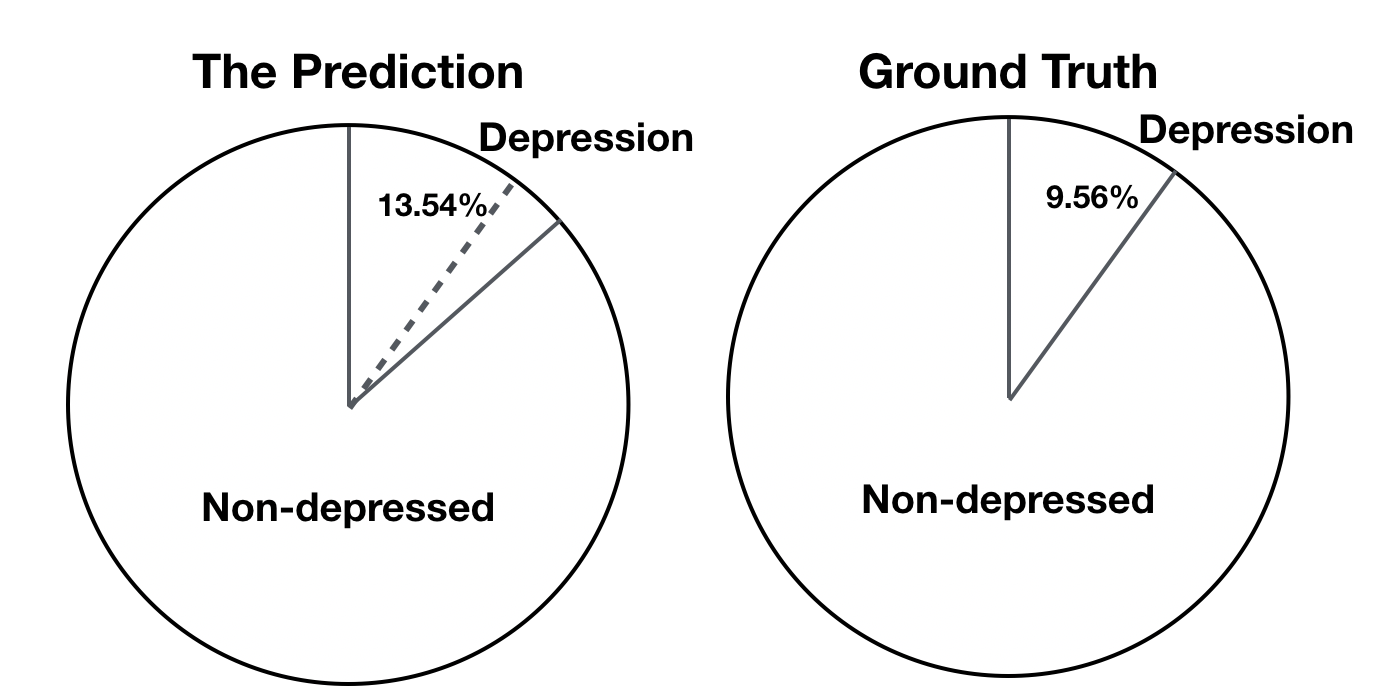
\includegraphics[width=1\textwidth]{coverage.png}
\caption{Coverage in correct classification of depression} \label{fig5}
\end{figure}
The coverage (see fig. 5) of depression cases is slightly larger than the real situation of mental health inventory. However, it is absolutely acceptable for large sampling that there is no missing of any depression case and only about 4\% of total cases have been incorrectly labelled as depression in the prediction. The proposed ensemble method is perfect for preliminary screening of major depressive disorder in order to provide limited cases for further clinical diagnosis while without missing any potential depression case. 
\\

In comparison with the predictions in the different sub-datasets (see table. 3), ensemble classifier performs the best in the overall dataset and has a similar accuracy in mental subset. The importance of diagnostic criteria in mental symptoms has been manifested that mental criteria are certainly the major features for identifying depression. Meanwhile, both accuracy and F1 measures for predicting depression in physical, social and role are equal to the predictive performance in general subset. However, general subset (70 features) has much more features than physical (7 features), social (6 features) and role (9 features) three subsets. It means that there are a lot of features in general subset occurred without enough specificity for classifying depressed and non-depression labels. Partial of general functional features hence are useless in the detection of depression. Correspondingly, features in physical, social and role functional subsets present more correlational in the classification. Weak depression indicator is not only helpless in the classification, but also incline the overall predictive accuracy. Therefore, it is extremely critical for depression diagnostic approaches to select a limited number of suitable features to distinguish depressed cases from a wide range. From the result of this research, we suggest an algorithm for feature selection which first involves as more mental symptoms as possible according to depression diagnostic criteria and pluses no more than 50\% features in health criteria in physical, role and social functionality. This algorithm ensures the majority of features consisted by metal diagnostic criteria and mixes partial health criteria to avoid the scenario that temporary mental status change occurs by sudden events like losing close relatives. It simulates the proceedings that psychologist did in the standard clinical interview. 
\\
\pagebreak
% =================================================================Future Work and Conclusion
\section{Conclusion And Future Work}
This work presented a binary ensemble system which is able to preliminarily distinguish depressive cases from a wide range of health data without the missing identification of any potential depressed case. In the experimental evaluation on NCHS dataset, only 4\% cases were mistakenly classified into depressed class and no depressed case has been detected incorrectly. The ensemble classifier on the whole dataset has a high F1 measure as 0.976 comparing to PHQ-9 depression screen inventory, 95.4\% and 95.6\% for Accuracy and Precision, respectively. It also demonstrated that the ensemble system is stable and robust for detecting depression on a partial of dataset. Moving forward, this research can help in preliminary screening of depressive cases from a large number of potential cases before formal clinical diagnosis. It is able to save huge cost in the psychological healthcare. It provides a much more efficient way to screen more people than traditional technologies and has a similar accuracy and coverage as current mental scale inventory. However, the reliability and sensitivity of this ensemble system need to be tested next on more datasets and text mining on social network platforms. In the conclusion, the presented work clearly illustrated the predictive capability of the proposed ensemble system to efficiently distinguish depressive instances from a board span of healthcare occasions.
\\

As future work, there are several future research directions of detecting depression that need to be carefully analysed for applying our ensemble system. One trend is to utilise rich online social media sources to extract features on the classification. It certainly will help improve the reliability and sensitivity of ensemble system. It hence will be our next work on the schedule.  Another interesting research direction is to examine images and brain EEG signals for mental clinic purpose. Deep learning has gained more momentum in such areas. Current ensemble system involves four supervised learning algorithms, however it will not suit for deep learning. In order to detect depression in intricate circumstance, deep learning technologies like DNN will integrate to increase the performance of ensemble system in future. As a major issue of automate depression detection, we will also consider how to simulate the proceeding of clinic diagnosis to improve the actions of effectively selecting mental diagnostic features. 

\goodbreak
% =================================================================reference
\pagebreak
\setlinespacing{1.66}
\bibliographystyle{amsplain}
\bibliography{xbib}


\end{document}

